\documentclass[a4paper,11pt]{article}


%% Language and font encodings
\usepackage[english]{babel}
\usepackage[utf8x]{inputenc}
\usepackage{colortbl}
\usepackage[T1]{fontenc}
\usepackage{listings}
\usepackage{color}

% CSS
\lstdefinelanguage{CSS}{
  keywords={color,background-image:,margin,padding,font,weight,display,position,top,left,right,bottom,list,style,border,size,white,space,min,width, transition:, transform:, transition-property, transition-duration, transition-timing-function},	
  sensitive=true,
  morecomment=[l]{//},
  morecomment=[s]{/*}{*/},
  morestring=[b]',
  morestring=[b]",
  alsoletter={:},
  alsodigit={-}
}

% JavaScript
\lstdefinelanguage{JavaScript}{
  morekeywords={typeof, new, true, false, catch, function, return, null, catch, switch, var, if, in, while, do, else, case, break},
  morecomment=[s]{/*}{*/},
  morecomment=[l]//,
  morestring=[b]",
  morestring=[b]'
}

\lstdefinelanguage{HTML5}{
  language=html,
  sensitive=true,	
  alsoletter={<>=-},	
  morecomment=[s]{<!-}{-->},
  tag=[s],
  otherkeywords={
  % General
  >,
  % Standard tags
	<!DOCTYPE,
  </html, <html, <head, <title, </title, <style, </style, <link, </head, <meta, />,
	% body
	</body, <body,
	% Divs
	</div, <div, </div>, 
	% Paragraphs
	</p, <p, </p>,
	% scripts
	</script, <script,
  % More tags...
  <canvas, /canvas>, <svg, <rect, <animateTransform, </rect>, </svg>, <video, <source, <iframe, </iframe>, </video>, <image, </image>, <header, </header, <article, </article
  },
  ndkeywords={
  % General
  =,
  % HTML attributes
  charset=, src=, id=, width=, height=, style=, type=, rel=, href=,
  % SVG attributes
  fill=, attributeName=, begin=, dur=, from=, to=, poster=, controls=, x=, y=, repeatCount=, xlink:href=,
  % properties
  margin:, padding:, background-image:, border:, top:, left:, position:, width:, height:, margin-top:, margin-bottom:, font-size:, line-height:,
	% CSS3 properties
  transform:, -moz-transform:, -webkit-transform:,
  animation:, -webkit-animation:,
  transition:,  transition-duration:, transition-property:, transition-timing-function:,
  }
}

\lstdefinestyle{htmlcssjs} {%
  % General design
%  backgroundcolor=\color{editorGray},
  basicstyle={\footnotesize\ttfamily},   
  frame=b,
  % line-numbers
  xleftmargin={0.75cm},
  numbers=left,
  stepnumber=1,
  firstnumber=1,
  numberfirstline=true,	
  % Code design
  identifierstyle=\color{black},
  keywordstyle=\color{blue}\bfseries,
  ndkeywordstyle=\color{editorGreen}\bfseries,
  stringstyle=\color{editorOcher}\ttfamily,
  commentstyle=\color{brown}\ttfamily,
  % Code
  language=HTML5,
  alsolanguage=JavaScript,
  alsodigit={.:;},	
  tabsize=2,
  showtabs=false,
  showspaces=false,
  showstringspaces=false,
  extendedchars=true,
  breaklines=true,
  % German umlauts
  literate=%
  {Ö}{{\"O}}1
  {Ä}{{\"A}}1
  {Ü}{{\"U}}1
  {ß}{{\ss}}1
  {ü}{{\"u}}1
  {ä}{{\"a}}1
  {ö}{{\"o}}1
}
%
\lstdefinestyle{py} {%
language=python,
literate=%
*{0}{{{\color{lightred}0}}}1
{1}{{{\color{lightred}1}}}1
{2}{{{\color{lightred}2}}}1
{3}{{{\color{lightred}3}}}1
{4}{{{\color{lightred}4}}}1
{5}{{{\color{lightred}5}}}1
{6}{{{\color{lightred}6}}}1
{7}{{{\color{lightred}7}}}1
{8}{{{\color{lightred}8}}}1
{9}{{{\color{lightred}9}}}1,
basicstyle=\footnotesize\ttfamily, % Standardschrift
numbers=left,               % Ort der Zeilennummern
%numberstyle=\tiny,          % Stil der Zeilennummern
%stepnumber=2,               % Abstand zwischen den Zeilennummern
numbersep=5pt,              % Abstand der Nummern zum Text
tabsize=4,                  % Groesse von Tabs
extendedchars=true,         %
breaklines=true,            % Zeilen werden Umgebrochen
keywordstyle=\color{blue}\bfseries,
frame=b,
commentstyle=\color{brown}\itshape,
stringstyle=\color{editorOcher}\ttfamily, % Farbe der String
showspaces=false,           % Leerzeichen anzeigen ?
showtabs=false,             % Tabs anzeigen ?
xleftmargin=17pt,
framexleftmargin=17pt,
framexrightmargin=5pt,
framexbottommargin=4pt,
%backgroundcolor=\color{lightgray},
showstringspaces=false,      % Leerzeichen in Strings anzeigen ?
}%
%
\makeatother
%% Sets page size and margins
\usepackage[a4paper,top=3cm,bottom=2cm,left=3cm,right=3cm,marginparwidth=1.75cm]{geometry}

%% Useful packages
\usepackage{amsmath}
\usepackage{graphicx}
\usepackage[colorinlistoftodos]{todonotes}
\usepackage[colorlinks=true, allcolors=blue]{hyperref}
\usepackage{indentfirst}

\title{Final Report}
\author{Written by : GoChat Team}

\definecolor{mygreen}{rgb}{0,0.6,0}
\definecolor{mygray}{rgb}{0.5,0.5,0.5}
\definecolor{mymauve}{rgb}{0.58,0,0.82}

\lstset{ %
  backgroundcolor=\color{white},   % choose the background color
  basicstyle=\footnotesize,        % size of fonts used for the code
  breaklines=true,                 % automatic line breaking only at whitespace
  captionpos=b,                    % sets the caption-position to bottom
  commentstyle=\color{mygreen},    % comment style
  escapeinside={\%*}{*)},          % if you want to add LaTeX within your code
  keywordstyle=\color{blue},       % keyword style
  stringstyle=\color{mymauve},     % string literal style
}



\begin{document}
\maketitle

%\begin{abstract}
%Your abstract.
%\end{abstract}

\section{Introduction}
Nowadays, with the rapid development of digital technologies, distributed instant messaging or chat systems, like Messenger of Facebook, WhatsApp and Telegram, play an increasingly indispensable role in people’s daily life. They provide an efficient way for people with geographical barriers to communicate, study, and work together conveniently.

In this report, we will describe the details of  our distributed chat system project, Go-chat. It consists of one server and two clients, Windows desktop application and web page. While C\# and PHP are chosen as the programming languages for the Windows desktop application and web page respectively, we decided to use Javascript in the server. Although go-chat is not as powerful as commercial chat applications, like WhatsApp, we hope that user will be able to enjoy their communication with each other on Go-chat. To begin with, a brief overview of our group project will be given. Then, related work about chat systems, requirements and design of our project and the most significant implementation details of go-chat will be described in details. After that, cooperation of our group and evaluation of our chat application will be demonstrated veritably and critically. Finally, the future works related to our project will be indicated in the end.






%WebSocket Protocol is used to ensure the communication between clients and server. (The WebSocket is a feature of HTML5 for establishing a socket connections between a web browser and a server, once the connection has been established with the server, all WebSocket data (frames) are sent directly over a socket rather than usual HTTP response and requests, giving us much faster, persistent and full-duplex communication between a web browser and a server.)





%\subsection{Project Scope}



\section{Review}
Instant messaging is one of the popular software application in human life in some counties. Van Vleck argued that its history is older than the Internet in 2012. In this session, history of Instant messaging can be defined into five stages.

The appearance of Compatible Time-Sharing System (CTSS) remarked the beginning in instant messaging. CTSS was invented at Massachusetts Institute of Technology (MIT) Computation Center in 1961. The initial purpose of CTSS was for offering convenience in education because it provides a new technic method for students to share information. By 1965, more than hundreds of users registered in CTSS. Most of them they were students of MIT and some colleges in New England. Furthermore, the Service allowed up to 30 simultaneous users on each of the Computation Center.  Students were encouraged to share information in different place. After they logged into MIT's IBM 7094, they not only send and receive messages but also creative and store files online on disk to share with each other.

In the 1970s, the creation of PLATO basic system was important stage in the evolution of instant messages as well as in the social dimensions, because it was one of the first online communities. In 1974, an online system named Talkomatic, which was been creative by Doug Brown. Compare other online chat systems, it is distinguished in that each user appears in their part of interface and messages are broadcast when user are typing, because most instant message post a message only after the message is already complete and the sender has clicked the send button. Soon after, PLATO’s use makes online chat more and more popular.  People start to focus on online communication. Talkomatic allowed that up to 5 five active Users text with each other in real time, by using a single a single Talkomatic channel and Channels could be created by any participators at any time. Besides, Users could prevent others action, like joining or observing, when a channel was created. Thereby, in some degree, people could creative private chat in their channels. 
 

America Online (AOL) is one of the biggest Internet providers at present. It provides an interactive service for public who desire to connect quickly and with lots of popular services, like the latest breaking news, gossip, sports, business and stock quotes on the web. AOL Instant Messaging system (AIM) was one of AOL’s most well-known services, born from May 1997. Initially, it was originally designed as a feature for AOL’s pay service. However, AIM quickly became the leading instant messaging application in the late 1990s early 2000s in North America. Basically, AOL is a text-based near-real-time application. When the users signed up and login AIM, users can maintain a list of contacts and can also sort their contacts into groups. The Interface not only shows the state of friends, online or logging out but also is alerted whenever one of those in the list comes on-line. The users can initiate a conversation session, type text messages and send an instant message to others. 

Extensible Messaging and Presence Protocol (XMPP), Instant Messaging and Presence Protocol (IMPP), Presence and Instant Messaging (PRIM) and SIP for Instant Messaging and Presence Leveraging Extensions (SIMPLE) are four predominant protocols of the instant message at present. XMPP is shown to be highly suitable for the network among the four protocols because it based on open Extensible Markup Language (XML) protocol, which inherits the flexibility of XML in a developed environment. Therefore, XMPP-based applications are with superior scalability. XMPP original name is Jabber. In 2000, open standards-based protocol named Jabber was launched by an open source organization. The protocol was standardized by Internet Engineering Task Force (IETF) and was renamed XMPP in 2002. 

XMPP server as an intelligent abstraction layer, it presents the client to deal with the XML data directly. In general, XMPP server should manage connections from authorized clients and could connect directly client applications and other entities. XMPP server is able to communicate with other XMPP servers. Due to XMPP servers and other associated services provide various of functionality and process kinds of data, so most clients just connect to a server over Transmission Control Protocol (TCP) in XMPP. As different system have the different protocol, gateway has to process and implement protocol conversation in XMPP for communication between XMPP and another system. On the whole, XMPP is an open, standard, proven, decentralized, secure, extensible, flexible and diverse protocol.

In this day and ages, using instant messages to communicate with others became predominant.
Although Messenger of facebook, Whatsapp and Telegram are the three of popular instant messaging at present.
They have their advantages to attract users, but they still left some place to improve.

The main function of an instant message is texts. These three instant message applications basically use Internet connection to send messages, so users can avoid SMS fees from mobile phone operators. When Users chat in the three instant messaging application, they could know that if their friend is type or not and they allow to have their usernames. What is more, Users of Messenger (Facebook) can see what time their messages are delivered and seen by their friends. Users only can know that the state of messages is delivered or seen in WhatsApp and Telegram. The contacts in Messenger (Facebook) are come from your friend's list in Facebook, while WhatsApp and Telegram are according your contacts in your phone and identify different users by their phone number. After a message was sent, sender still can edit that message only in Telegram, and the message will be marked that what time it was edited. As a result, Telegram performs better than Messenger (Facebook) and WhatsApp in this basic function.

Sending voice messages is becoming a second basic function is instant message system. Sometimes, users are on the go or just do not have time to type messages and longer story, so users could choose to record their voice and send the voice messages in this situation. Generally, this function is preferred for the old people or some people who do not how to typing. It is a significant reason, why instant message application has huge ranges of users. Messenger (Facebook), WhatsApp and Telegram, these three instant message applications, all of them support this function. The little different thing is that when the receivers listen the voice, the users could choose the begin time of voice messages to listen in WhatsApp and Telegram. However, users have to listen whole records in Messenger (Facebook), when they listen any voice messages. In this case, if users miss or confused on last 10 seconds records in a 5 minutes voice messages, they have to spend 5 minutes listen the voice message again, rather than just listen last 10 seconds again. In brief, WhatsApp and Telegram do better than Messenger (Facebook) in voice messages part.

One-to-one chat is no longer satisfied people ‘s requirement in communication in their normal life. For this reason, users could start a group chat with their contacts, aiming to keep in touch with groups of people, like your family members, classmates, coworkers. When users chat in a group, they could mention some members in their messages, and members could reply any single record in history. The difference about group chat is the up bound of number of group members. Messenger (Facebook) is quite weak and limited because it only allows less than 50 people in one group. Users of WhatsApp could communication with up to 256 contacts in one group. Compared Messenger (Facebook) and WhatsApp, Telegram show its are extremely powerful in group chat function. The telegram can hold up to 5000 members in each chat group. Moreover, Telegram owns another attracting related function, called Channels. Channels are much more like a broadcast, broadcasting public messages to large audiences. Channels are essentially broadcasting to a larger audience and it can hold unlimited members. It is much suitable for some supervisor-subordinate communication or official speech. So when users post in a channel, the publisher of messages is signed with the channel's name and photo.  

Share Location, this function is a much helpful function in human real life rather than Internet life. Most of people had ever tried to give directions to somebody, if the people do not sure their location or their friend do not have sense of direction, it will become a frustrating experience. However, Users could send their exact location to their contacts and instantly update the current location in Messenger (Facebook) WhatsApp and Telegram, so this instant messaging application help users to save time and avoid people get lost in some degree. Therefore, this function, Share Location, contribute to user’s meeting in real life.

Users of Messenger (Facebook) and WhatsApp can communicate with others by voice calls or face-to-face conversations when text just isn't enough. The free voice calls and video calls are available when the application connects the Internet. Therefore, people don't have to worry about expensive calling charges if their contacts are in other countries. However, Telegram has not this function at present.


Telegram maximizes its strong advantage in the function of Send Files. Send files means that users could send documents; pictures, video and more directly in chat interfaces through the instant messaging application, without the hassle of email or others application.  On the one hand, users can share size of files up to 1.5GB in Telegram, but the maximum file size upload for WhatsApp and Messenger (Facebook) is only 100MB and 25MB separately. On the other hand, users could share almost any file types including documents, zip, PDF etc. in Telegram. However, WhatsApp and Messenger (Facebook) limit the type of documents. Users recently included the ability to send PDF in WhatsApp. To summarize, WhatsApp and Messenger (Facebook) do no match to Telegram’s file sharing abilities.

These three instant message applications support most of the mainstream clients. WhatsApp initially is available on mobile devices (such as IOS, Android and Windows). At present, it is offering web and desktop clients for Mac and Windows, too. Comparatively, Messenger (Facebook) and Telegram even have desktop clients for Linux. In details, Messenger (Facebook) and Whatsapp do better than WhatsApp here. The fact is that these two applications offer independent apps for all platforms.  However, the mobile application should be   running, if users work WhatsApp in the desktop and web clients.

In recent year, the crisis in individual privacy and trade secret occur frequently. It encourages people set out to take information security more seriously. Hence, each application developer has to pay more attention to information security for enhancing the degree of belief from customs. In last year, WhatsApp created the largest end-to-end encrypted messaging network in history, because of a new layer of security over all chats and data like text messages, voice messages even media to billion users’ applications. After this end-to-end encryption, it means that only senders and receivers can read their chats, even the WhatsApp cannot read it. Messenger (Facebook) just finished rolling out “Secret Conversations” which uses the Signal encryption system. Although it has not explicitly mentioned this new function on users’ device, users could create secret chats by their selves. Nevertheless, the function, “Secret chats” with end-to-end encryption, is known as a basic and essential function in Telegram. Telegram is based on their encryption protocol, which called MTProto Mobile protocol. Furthermore, users also could know if opposite side using screenshot on the chat interview by notifications. On the other hand, Telegram, as an open-source application, encourages everyone checks its source code and API. If someone finds any security flaws, Telegram will offer \$200,000 as an award. Consequently, the three applications all make efforts and contribution to users communication security.


\section{Requirement and Design}
\subsection{Requirement}
The requirement for this project is to build a reliable, secure, and attractive chat system. Reliable in the term that every message sent by the client will receive in a relatively real-time. The client would not have to concern about lost message even in a slow network connection or offline case. Meanwhile, secure in this case means that there is no unauthorized principal can read a message sent from one client to another client.

According to the requirement, we divided our project into three main level, Basic Chatting Program, Security, and Other Additional Functions. 
\subsubsection{Level 1: Basic Functionalities}
In this level, basic infrastructure will be built for the server and two clients, the web page and the Windows desktop application, to achieve basic functionalities for the system. 

\begin{itemize}
%--------------------------------------------------------
%change User




\item Server
\begin{enumerate}
\item  Since storing chat messages and retrieving those messages at a very fast rate is much needed for a chatting software, the MYSQL is used as our database management system, and four tables are needed to be created to store different sorts of data (Figure 1).

\begin{figure}[h!]
\centering
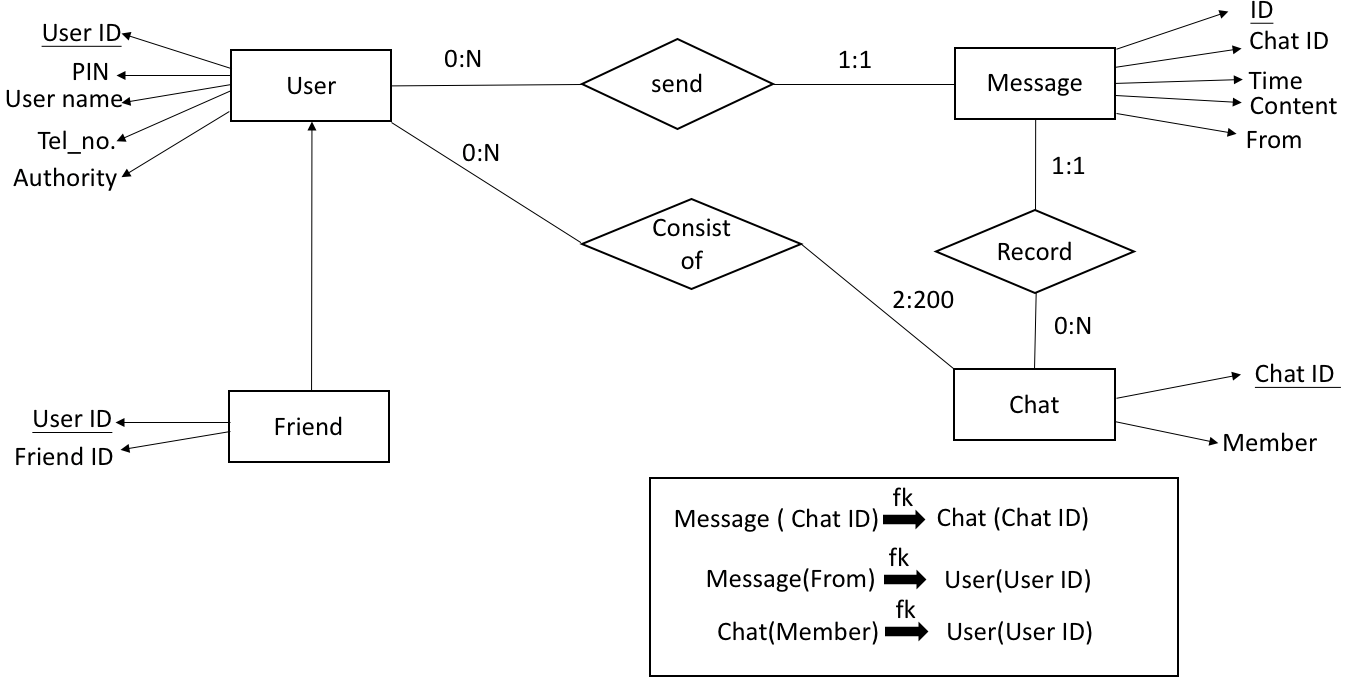
\includegraphics[width = 0.8 \textwidth ]{ERD.png}
\caption{\label{fig:ERD}Previous Vision of E-R modeling}
\end{figure}
\begin{figure}[h!]
\centering
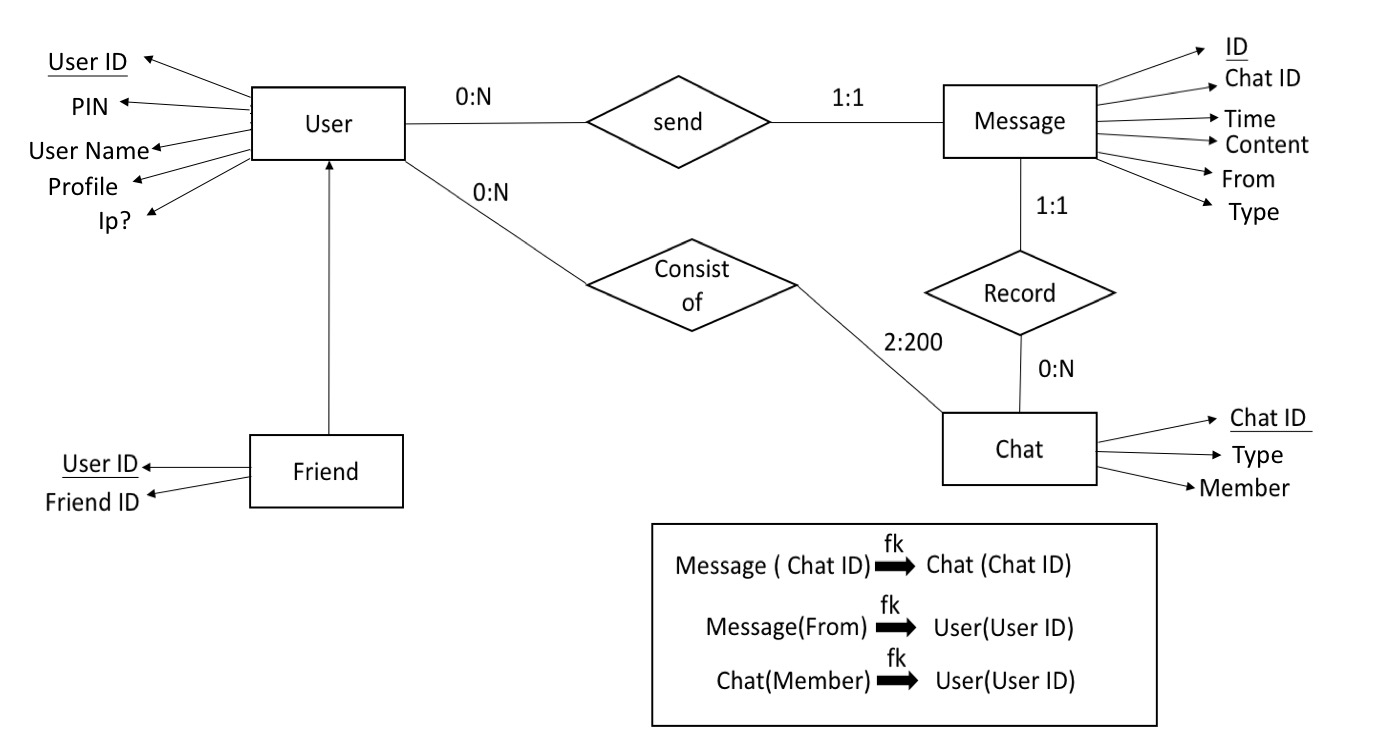
\includegraphics[width = 0.8 \textwidth ]{current-erd.jpeg}
\caption{\label{fig:ERD}Current Vision of E-R modeling}
\end{figure}
\begin{itemize}
\item 
\item Table ‘user’ would contain the basic information of all users including userID, password, username, prfile and Ip. Ip address will be insert into database only if the user is online.
\item Table ‘friend’ is used to store the userID and the friendID of their friends’.
\item Table ‘message’ will list the detail of every single message including chatID, sending time, a content of the message, userID of sender and the type of the message (file,image,text etc.).
\item Table ‘chat’ is used to record the member of chatting and their chatID. Furthermore, the attribute of type is used to identify whether it is group chat or not. 
\end{itemize}



\begin{itemize}
\item Key constraint:

Primary key: user(userID), message(ID), friend(userID), chat(chatIÅD).

Foreign key: message(chatID), message(from), chat(member).

\end{itemize}

\item The Javascript server is used to make a connection between two clients based on WebSocket protocol.
\end{enumerate}


%: Keep chatting record in the database. It store data until the user request to delete history.

%: describe database table(how to store data)

%: it might be depend on option. If someone do not want to store data(like private mode), data will delete when user delete chatting.

% : open web sever by open source program Apache

% : it can be replace by github(github provide storage. it can use as a web server)


\item Client
\begin{enumerate}
\item Clients could set up the connection with server.
\item Client 1 sends message to server
\item Client 2 receive the message from the server which from the client 1.
\item Client 1 could send files or images to client 2 through server. 
\item Client 1 sends file path or image path in a given format to server with uploading it to the server. 
\item Then the server sends this file path or image path to client 2.
\item Client 2 download the file or image from the path.
\end {enumerate}
\item User

\begin{enumerate}

\item Users on the clients could sign up creating their user names and passwords and also filling in their personal details in sign up part.
\item Existing users on the clients could login with their name and passwords in login part. 
\item Users on the clients could add their friends and send messages (text, files and pictures) to them in chatting part.
\item Users on the clients could check whether their friends are online or not in chatting part.
\item  Users on the clients could create groups with adding their friends to the group and begin group chats in chatting part.

\end{enumerate}
\end{itemize}

%\begin{table}[h]
%\caption{Payload}
%\begin{center}
%\begin{tabular}{| c | c | c | c |}
%\hline
%sender & receiver & type & message\\
%\hline
%\end{tabular}
%\end{center}
%\end{table}

% \begin{itemize}
% \item Payload

% - This is a simple version of the payload for communicating between server and client

% - type: provide what type of the message it is. Such as plain text, picture, video, and document.

% - message: If message is a plain text, it contains the text. Another cases (picture, and so on), it contains server storage a URL. Based on the URL, files will be download from the server. 

% \end{itemize}
\subsubsection{Level 2: Security}

Chatting program is a private communication tool. Confidentiality, availability, and Integrity are three common issues at the chatting program. To minimize the possibility of compromise security issues, we focus on two parts, communication security and security of data storage.     

The data stored in database contains personal information, photos, business secret, and so on. This kind of information must be protected to avoid leakage. In level 1, program stores unencrypted chatting history at the server. Meanwhile, in level 2, it is encrypted by symmetric algorithm with securely stored keys. Thus, only those who participate in the chatting can read their chatting history from the database in the server with decryption of these information. In this case, even if there is a data leakage, attackers could not get any useful information about the users from this. In this level, the user also could delete their chatting history to prevent data leakage. In addition, user can customise message expire time. For example, if user set the expire time to one day, the message will be automatically deleted after 24 hours. The message will be deleted even if the receiver has not seen the message. To encrypt the user names and password to avoid dictionary attacks, we choose to use SALT and hash function. 

For communication security, WebSocket protocol can not be used to deal with the authorization or authentication. However, just like the HTTPs which is HTTP over TLS, using the WSS (WebSocket over TLS/SSL) to encrypt our connection can make sure our information transfer security. In this case, we just need to configure TLS encryption for WebSocket and self-sign the certificate.

\subsubsection{Level 3: Other Additional Functionalities}

Chatting program has to be attractive. It is not only for sending plaintext messages to friends. It must be possible for the application to express emotion of people. That's why people use emojis and photos. In level 3 period, go-chat program contain attractive function including using emojis, gif, drawing picture, recommending friend, offline message, printing history, recalling the message, and image compose.

\subsection{Design}

\subsubsection{Project Structure}

\begin{figure}[h]
\centering
\includegraphics[width = 1 \textwidth ]{time.jpg}
\caption{\label{fig:UML}Sequence Diagram}
\end{figure}

\begin{figure}[h]
\centering
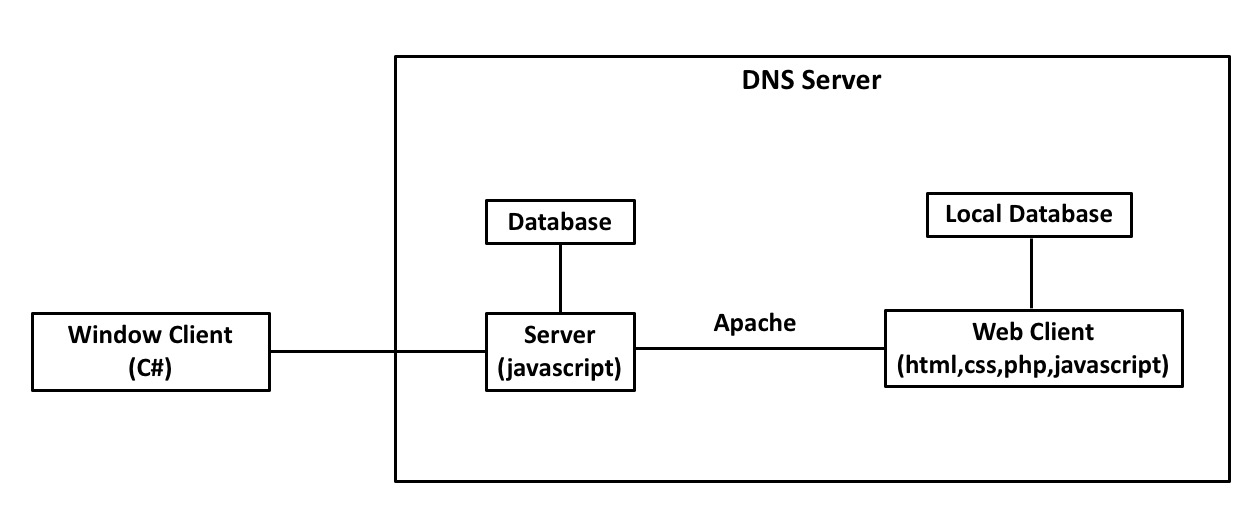
\includegraphics[width = 0.8 \textwidth ]{program_structure.jpeg}
\caption{\label{fig:UML}Program Structure}
\end{figure}




%-----------------------------------------------
% add some description 














\section{Implementation}
\subsection{Server}
\subsubsection{Connection with Main Database}
As we me mentioned above, we have two database in our infrastructure. The main database and local database which connected to server and web client respectively. We use node.js to create a connection between server and main database.
\begin{lstlisting}[language=javascript]
var mysql = require('mysql');
var conn = mysql.createConnection({
    host: 'localhost',
    user: 'root',
    password: '',
    database: 'gochat',
    port: 3306
});
conn.connect();
\end{lstlisting}
\subsubsection{Global Variables}
We declared a global variable ‘clients[ ]’ which plays an important in achieving functions. 
\begin{lstlisting}[language=javascript]
//Global variables
var clients = [ ];
\end{lstlisting}
The content of this global variable is message sent by online users, which means, in this way, ‘client[ ]’ is used to list the connected user. Take an example of how global variable takes part in process of function. When user login, server will receive the message of username and password. After that, the IP address of the user will be inserted into the database. Equally, the IP address will also be deleted after the user logs off. Server will depend on whether the user’s IP address is stored in the database to identify the online user.  
\begin{lstlisting}[language=javascript]
function InsertIp(Ip,UserName)
{
    conn.query('UPDATE user set Ip="'+Ip+'" where UserName="'+UserName+'"',
 }
 
var index=clients.push(connection) - 1;

InsertIp(clients[index].remoteAddress,UserName);
\end{lstlisting}
In terms of the code above, all the message sent by the online user will be pushed into the global variable, and the variable ‘index’ plays a part of counter. In this case, the IP Address would be got from the global variable and inserted into database according to the username.
\subsubsection{Design of websocket}
The most different thing between websocket and http protocol is that websocket provides full-duplex communication which means the communication between the server and client can be delivered in both direction simultaneously. In our server we choose 1337 as our websocket server port.
\begin{lstlisting}[language=javascript]
var webSocketsServerPort = 1337;
\end{lstlisting}
There is a callback function will be called when someone tries to connect to the websocket server. As the function running, server should check the ‘request.origin’ in order to make sure the client is connecting from the website. After that, server will send a message to the web console to inform that the connection has be established.
\begin{lstlisting}[language=javascript]
  console.log((new Date()) + ' Connection from origin ' + request.origin + '.');
\end{lstlisting}
\begin{lstlisting}[language=javascript]
  console.log((new Date()) + ' Connection accepted.');
    for (var i = 0; i < clients.length; i++) {
        console.log(i+"!!!!!"+clients[i].remoteAddress);
    }
\end{lstlisting}
\subsubsection{Message identification}
There are lots of different type of message received by server, for example, chatting message, registration, and adding friend. Therefore the way of how to identify the message is quite important. In our project, all the messages delivered as the format of JSON like the following code.
\begin{lstlisting}[language=javascript]
var str ="register$user$"+user+"$"+passwd+"$profile";
var str="message$"+ChatId+"$"+time+"$"+leftText+"$"+userId+"$0";
\end{lstlisting}
As shown above, the first word of the string is the type of the message, and all the data are linked by \$. In this way, server just needs to split the string through identifying the symbol of \$, and decide which service that the client wanted through checking the first element.
\begin{lstlisting}[language=javascript]
var strs = message.split('$');//SPLIT MESSAGE
if(strs[0] == "register")//REGISTER FUNCTION
        {
        conn.query('select * from user where UserName="'+strs[1]+'"',
        function(err, rows, fields) {
        if (err) throw err;
        if(rows.length>0){
            obj="please change another username";
            var json = JSON.stringify({type: 'register', data: obj});
            clients[index].sendUTF(json);
            }else{
              obj="succeed";
              var json = JSON.stringify({type: 'register', data: obj});
              clients[index].sendUTF(json);
                 }
          });
         }
\end{lstlisting}
\subsubsection{Password Hashing}
The most important aspect of a user account software is how user’s passwords are protected. Because database is frequently hacked, we must do something to make sure the security of our database. In this case, using hash function is an appropriate way to deal with our user’s password.

Hashing provides functions for generating a hashed passwords and verifying a plain-text password against a hashed password. The output of the hash function is fixed no matter what size of the password inputted. For a bit of added strength of hash value, a random salt is generated and added in front of the password, then hash the whole string. There are two reasons to add a random salt. For one thing, two equal will generate two totally different value, for another, there are already a huge amount of hash value have been disclosed, so that, adding salt can prevent the dictionary attack.

In our project, we use the 'node-forge' library to hash user’s password. Regarding how to generate the salt, the 'random.getByresSync' function is used to create a 64 bytes of salt.
\begin{lstlisting}[language=javascript]
var salt = forge.random.getBytesSync(64);
\end{lstlisting}
We used PBKDF2 algorithm with SHA256 as the base algorithm by calling ‘forge.pkcs5.pbkdf2’ function to hash the password and salt. This algorithm hashs the SALT and password repeatedly as an effort to enhance the security. In this project, we used 1000 iteration to hash password. The hash value and salt should be transfer from byte to hex using 'forge.util.bytesToHex'.
\begin{lstlisting}[language=javascript]
var key = forge.util.bytesToHex(forge.pkcs5.pbkdf2(strs[2], forge.util.bytesToHex(salt), iteration, 32,'sha256'));
\end{lstlisting}
The hash value will be stored in database in follow format:
\begin{lstlisting}[language=javascript]
var storedHash = forge.util.bytesToHex(salt)+ "$" +key;
\end{lstlisting}

\subsection{Window Desktop Client}
\subsubsection{UI Design}
There are five forms constituting the Gochat windows desktop application, login form (Figure5), sign up form (Figure6), chat form (Figure 11 ), add friends form (Figure 7) and create new group form (Figure8 ). In login form, existing users could type user name and password to login while new users could click new user label to sign up in sign up form. In sign up form, users could choose their profile photos from local folders, user names and passwords. If the re-password are not the same as the password, a message box will pop up to warn the user to retype the same password. 

\begin{figure}[h!]
\centering
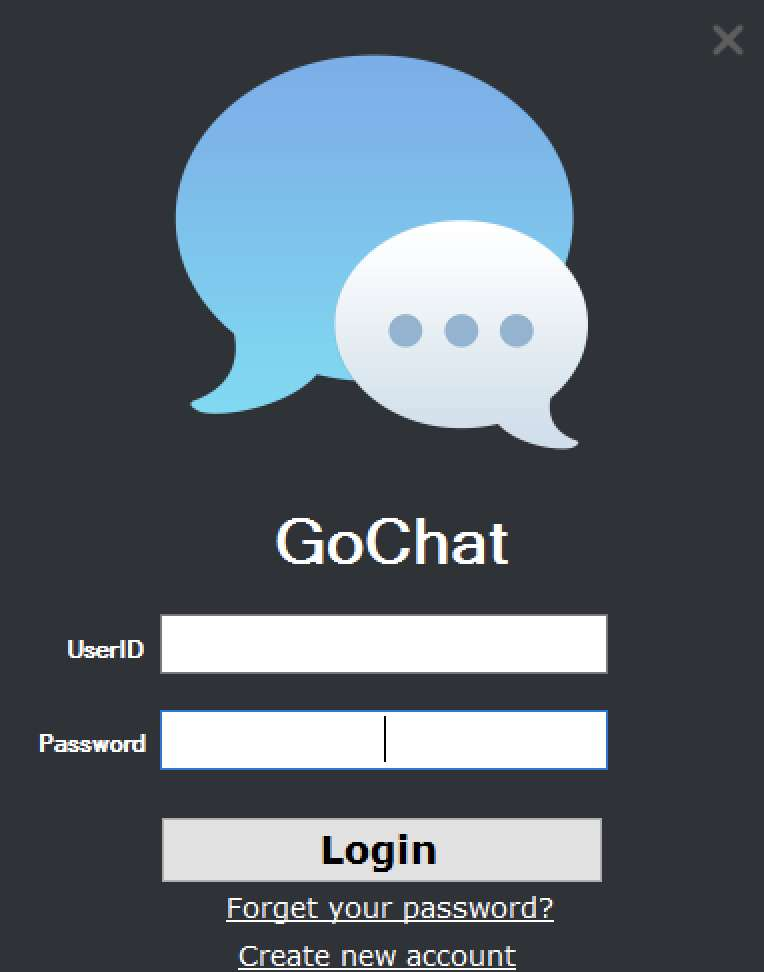
\includegraphics[width = 0.5 \textwidth ]{login_form.jpg}
\caption{\label{fig:UML}Login Form Chat}
\end{figure}

\begin{figure}[h!]
\centering
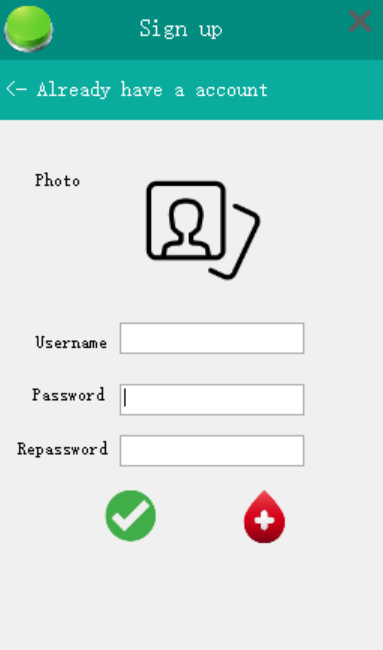
\includegraphics[width = 0.5 \textwidth ]{SignUpForm.PNG}
\caption{\label{fig:UML}Sign Up Form }
\end{figure}

\begin{figure}[h!]
\centering
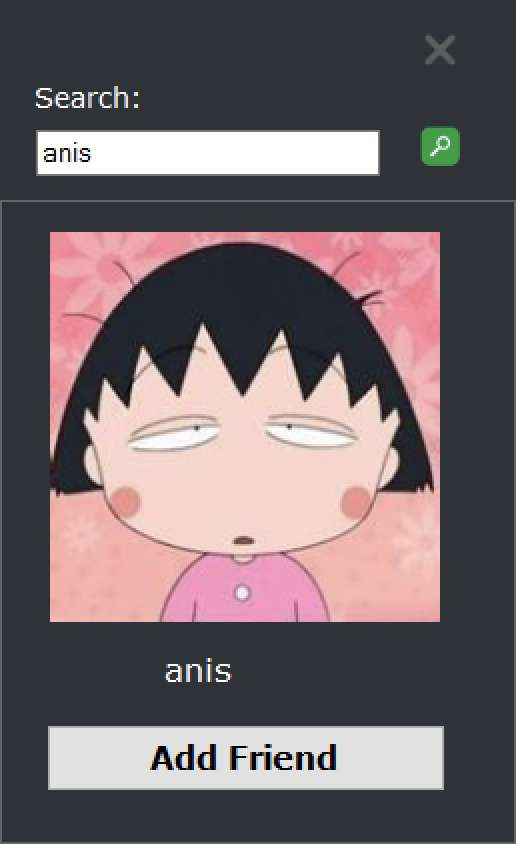
\includegraphics[width = 0.5 \textwidth ]{addFriendForm.jpg}
\caption{\label{fig:UML}Add Friends Form}
\end{figure}

\begin{figure}[h!]
\centering
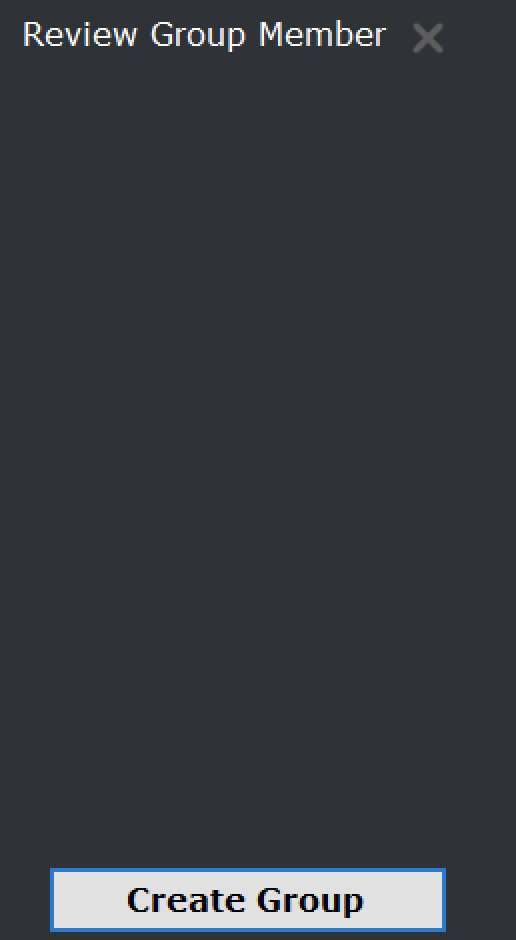
\includegraphics[width = 0.5 \textwidth ]{addGroupForm.jpg}
\caption{\label{fig:UML}Create New Group Form}
\end{figure}

\begin{figure}[h!]
\centering
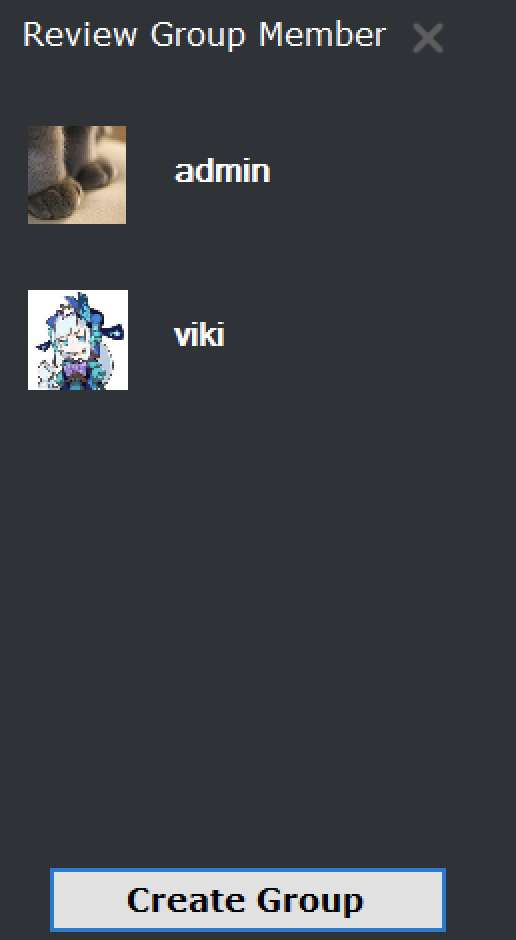
\includegraphics[width = 0.5 \textwidth ]{create_group_2.jpg}
\caption{\label{fig:UML}Create New Group Form 2}
\end{figure}

\begin{figure}[h!]
\centering
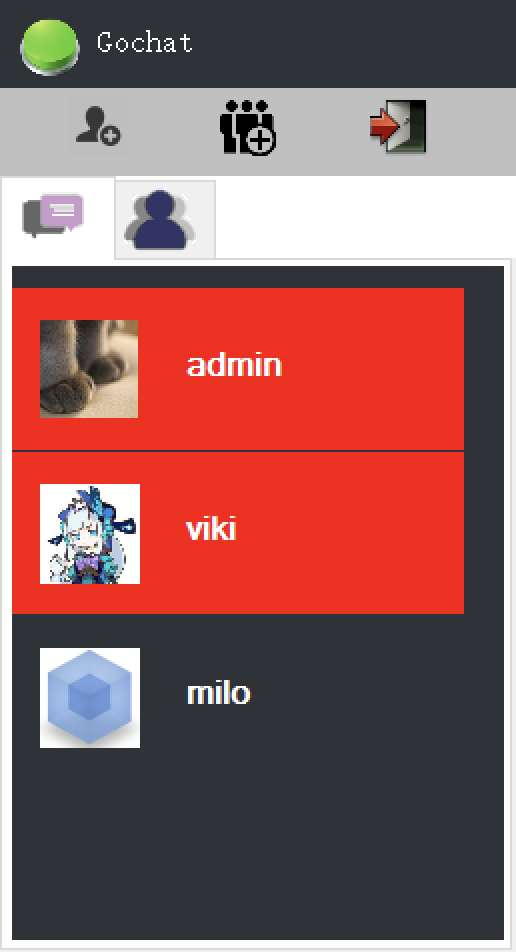
\includegraphics[width = 0.5 \textwidth ]{create_group3.jpg}
\caption{\label{fig:UML}Create New Group Form 3}
\end{figure}

\begin{figure}[h!]
\centering
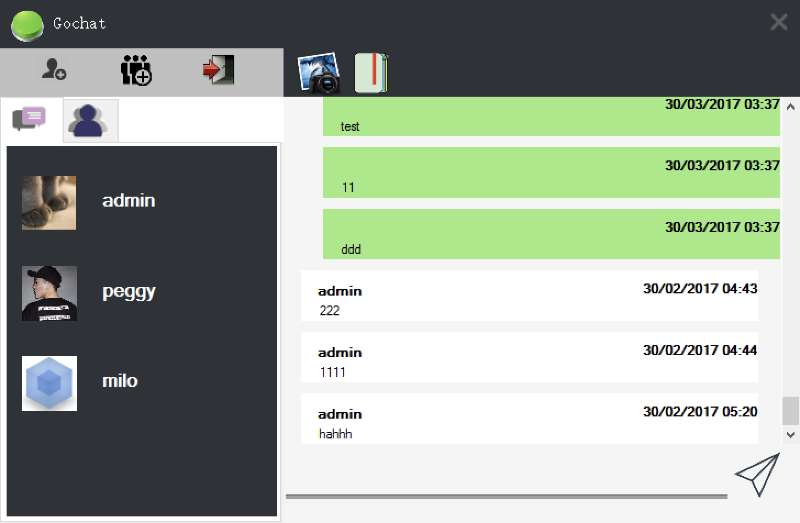
\includegraphics[width = 0.5 \textwidth ]{message.jpg}
\caption{\label{fig:UML}Chat Form}
\end{figure}

The chat form is separated into two parts, the list form and message form. After users login, the list form will show out. It is shown in Figure that there is a control panel in list form providing buttons for users to add friends, create groups and sign out. When the user clicks add groups button, the add groups form will be displayed. The user could select the existing group to add new members or select friends in the friend list to create a new group by clicking friends in the friend list or group in group list. After that, those friends or groups will appear in the add groups form. With clicking add group button in the form, a new group will be created and shown out in the group list. 

When the user clicks the add friends button, the user could see the add friends form. The user could type in the user name he or she want to search and click search button, the profile image and the user name will appear. Then, if the user clicks add friend button, this friend will be added and shown in the friend list.

In the list form, users can see friend list, group list and chat list by click different buttons. When users click a friend, a group or a chat from the list section, all chatting history will display in message window. Also, on the bottom of the message window, users could type and send the messages. On the top, images or files could be sent as well by clicking the corresponding picture buttons. 

\subsubsection{Connecting to Server}

As we mentioned before that we used WebSocket to connect server and clients. We used library provided by Microsoft Visual Studio to use WebSocket services. Basically we created a socket to communicate with server by providing its IP address and PORT. A cancellation token cts\_timer is defined and used in await function to end the setting up connection thread. The other one, cts, is defined and also used in await function to end the receive data thread.
\begin{lstlisting}[language=C]
public async Task StartAsync()
{
            cts = new CancellationTokenSource();
 CancellationTokenSource cts_timer = new CancellationTokenSource(10000);
            socket = new ClientWebSocket();
            string wsUri = "ws://47.91.75.150:1337";
            await socket.ConnectAsync(new Uri(wsUri), cts_timer.Token);
            Task.Factory.StartNew(
            async () =>
            {
                while (true)
                {
                    WebSocketReceiveResult rcvResult =
                    await socket.ReceiveAsync(rcvBuffer, cts.Token);
                }
            }, cts.Token, TaskCreationOptions.LongRunning,
                TaskScheduler.Default);
}
\end{lstlisting}
\subsubsection{Receiving Data from Server}

	Our windows client should be able to handle data in JSON format because the server that we build is in JavaScript. Thus, we need a library to translate JSON format data into an object in C\#. The library that we used was 'Newtonsoft.Json.dll'. This library makes it easier to transform JSON data into a class. For example, we used this code below to transform JSON data 'rcvMsg' into an object 'NewUserTable'.

\begin{lstlisting}[language=C]
string rcvMsg = "{\"type\":\"user\",\"data\":{ \"UserId\":3,\"PIN\":\"admin\",\"UserName\":\"peggy\",\"profile\":\"assets / dist / images / 5.jpg\"}}";

public class UserTable
        {
            public string type { get; set; }
            public user data { get; set; }
        }

public class user
        {
            public int UserId { get; set; }
            public string PIN { get; set; }
            public string UserName { get; set; }
            public string profile { get; set; }
        }
        
public UserTable NewUserTable = new UserTable();

NewUserTable = JsonConvert.DeserializeObject<UserTable>(rcvMsg);
\end{lstlisting}

When a user login, windows client will send username and password to server for verification process. After server verify the user, it will send four JSON objects to client. These objects contain all user's chat histories stored by server.

\begin{table}
\centering
\begin{tabular}{l|l}
\hline
Object & Content  \\\hline
User & Details of user  \\\hline
Friend & Friend's details  \\\hline
Chat & All chat histories belong to user  \\\hline
Message & All messages belong to related chat histories  \\\hline
\end{tabular}
\caption{\label{tab:json}Objects Sent by Server}
\end{table}

By using the previous code, we can easily transform these JSON objects into C\# supported objects and use them in required functions. 

\subsubsection{Sending Data to Server}

When we want to send data to server, we have to follow a certain template. This template will make sure that server recognize our data and store them in correct table in the database. 

\begin{lstlisting}[language=C]
type\&column\&column\&...\&column
\end{lstlisting}

For example, when userA want to send message to userB, instead of sending the content directly, windows client will send it following this template:

\begin{lstlisting}[language=C]
message\&chatId\&time\&content\&from\&type
\end{lstlisting}

Therefore, the server can store this data in 'message' table and forward it to userB.


\subsubsection{List and Message Display}
User control item named chatmesg is embedded into another user control item called chatbox to display every single message. When new message is sent or received, new user control item will be generated and displayed below the preview ones. Chatmesg, textbox, send message button, select image and file buttons are combined together in chatbox user control item and embedded into chat form. Likewise, user control item, friend item is used to display each chat or group in the list form and also embedded into friend list user control item. The friend list user control item is embedded into chat form at the end.  
When we display chat list, we want to do two different things. First, we want to get chat ID from all the chats with type = 0 in object 'chat'. Then, we want to display the username of friend who involve in the chats.
We can display group chat by filtering all the chats that have type = 1 from object 'chat'.
We can display friend list simply by displaying all data from object 'friend'.




\subsubsection{Add Friends, Create a New Group or User}
\begin{itemize}
\item Add Friends

\begin{figure}[h!]
\centering
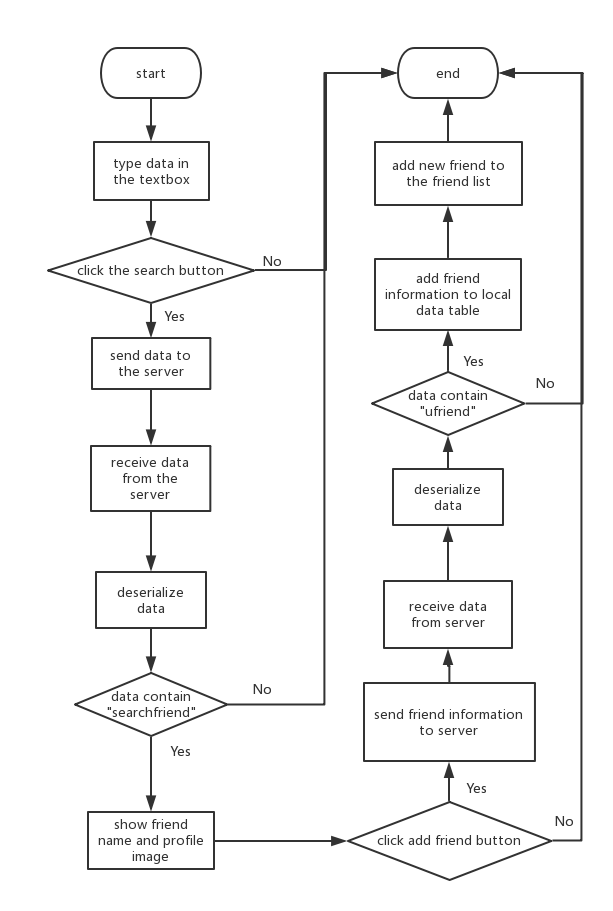
\includegraphics[width = 0.8 \textwidth ]{add_friend_flow_chat.png}
\caption{\label{fig:UML}Login Form Chat}
\end{figure}


As shown in Figure 12, after the user type a user name who he wants to search and then click search, data will be sent to the server. The codes for getting data from the text box in add friend form and sending it to login form to call the function to send the data to the server are given as follow.

\begin{lstlisting}[language=C]
//Search friend form
private void pictureBox1_Click_1(object sender, EventArgs e)
        {
            MainForm.searchUser(textBox1.Text);
        }
//Form 1
internal void searchUser(string str)
        {
            loginForm.searchFriend(str);
        }
//Login form
 public void searchFriend(string str)
        {
            string message = "search" + check + userinfo.UserId + check + str;
            send_data(message);
        }
\end{lstlisting}
And then, window client will receive data form the server and deserialize it. After that, the user name and profile image will be displayed in search friend form. The codes for these steps are given:

\begin{lstlisting}[language=C]
//Form 1: send data to search friend form
internal void sendUserInfo(Login.user temp)
        {
            SFriend.userdetail_fromLogin(temp);
        }
//search friend form:show user name and profile image out 
internal void userdetail_fromLogin(Login.user temp)
        {
            userDetail2.setUserData(temp);
        }
        internal void setUserData(Login.user temp)
        {
            this.UserData = temp;
            set_image(temp.profile);
            set_userName(temp.UserName);
        }
\end{lstlisting}
When the user clicks add friend button, the friend information will be sent to the server and then server will send the new friend list back to the client. The client will add this new friend to local data table and also update it in the friend list.



\item Create a New Group

The process of creating a new chat or group function is similar as adding friends function. Compared to adding friends function, the difference of creating a new chat or group is that a string list is defined to store the user ID of the friend or members in the group chose by the user. The codes are given as follow:

\begin{lstlisting}[language=C]
//define the string list 
private void addGroupButton_Click(object sender, EventArgs e)
{
strfriendList = new List<string>();
}
//add user ID to the list
public void friend_item_Click(object sender, EventArgs e)
{
        MainForm.add_strfriendList(this.userID.ToString());
}
public void add_strfriendList(string str)
{
            strfriendList.Add(str);                   
}
// remove duplicate user ID in the list 
 public void passMemberID()
{
        string temp = loginForm.userinfo.UserId.ToString();
            foreach (string s in strfriendList)
            {
               temp += "," + s;                
            }
            var temp1 = temp.Split(',').ToList();
            var temp2 = temp1.Distinct().ToList();
            var sortemp2 = temp2.OrderBy(x => x).ToList();
            string memberID = String.Join(",", sortemp2);
}

\end{lstlisting}

\item Create a New User

The process of creating a new user or signing up is also similar as adding friends. The difference is that the user could choose his profile image and  its file path will be sent to server. And also the connection is started by 
newConnectWs function. (In adding friends and creating a new group part, the connection is already started when the user login.)
\begin{lstlisting}[language=C]
//select the profile image 
  private void pictureBox3_Click(object sender, EventArgs e)
{
            OpenFileDialog dlg = new OpenFileDialog();
            dlg.Filter = "JPG|*.jpg|GIF|*.gif|PNG|*.png|BMP|*.bmp";
            dlg.Title = "File Sharing Client";
            dlg.ShowDialog();
            //txtFile.Text = dlg.FileName;
            fileName = dlg.FileName;
            photo.ImageLocation = fileName;
}
//sending data to the server
private void pictureBox5_Click(object sender, EventArgs e)
        {
            this.loginForm.getSendMessage = UName.Text;
           this.Invoke(new createAccount(loginForm.createNewAccount), username, password, profile);
            loginForm.newConnectWs();
        }
\end{lstlisting}

\end{itemize}










\subsection{Web Client}

\subsubsection{Frameworks}
As mentioned previously, our web client is using Model-View-Controller(MVC) software architectural pattern, which is a quite popular framework for designing web applications. Using MVC can achieve the simultaneous development of software because developers are able to work in different tiers without influence each other, and that is why we choose it for this group project. In this project, we choose the CodeIgniter as our framework of the web client.

\subsubsection*{View Tier}
The viewis a software class that contains a template and data form and produces a response for the browser. It receives data from the Controller of the MVC and packages it and presents it to the browser for display.

We have two forms in the view tier. One is the chatting form which is used to show the main interface of the web client. The other is login form which is for log in function and registration of a new account. After logging in, the user can see the whole chatting window. The interface is divided into three main parts. The sidebar, which located on the left side, displays all the basic information about user’s account, for example, friend list, group chat list .etc. There is an option bottom on the top right corner of the sidebar which contains three functions: add friends, create group chat and log out. The right of the interface is message window and text window, which are used to display the chatting history and input the message respectively. We used many icons to represent the related functions that are easier to be understood by users. 

\begin{figure}[h!]
\centering
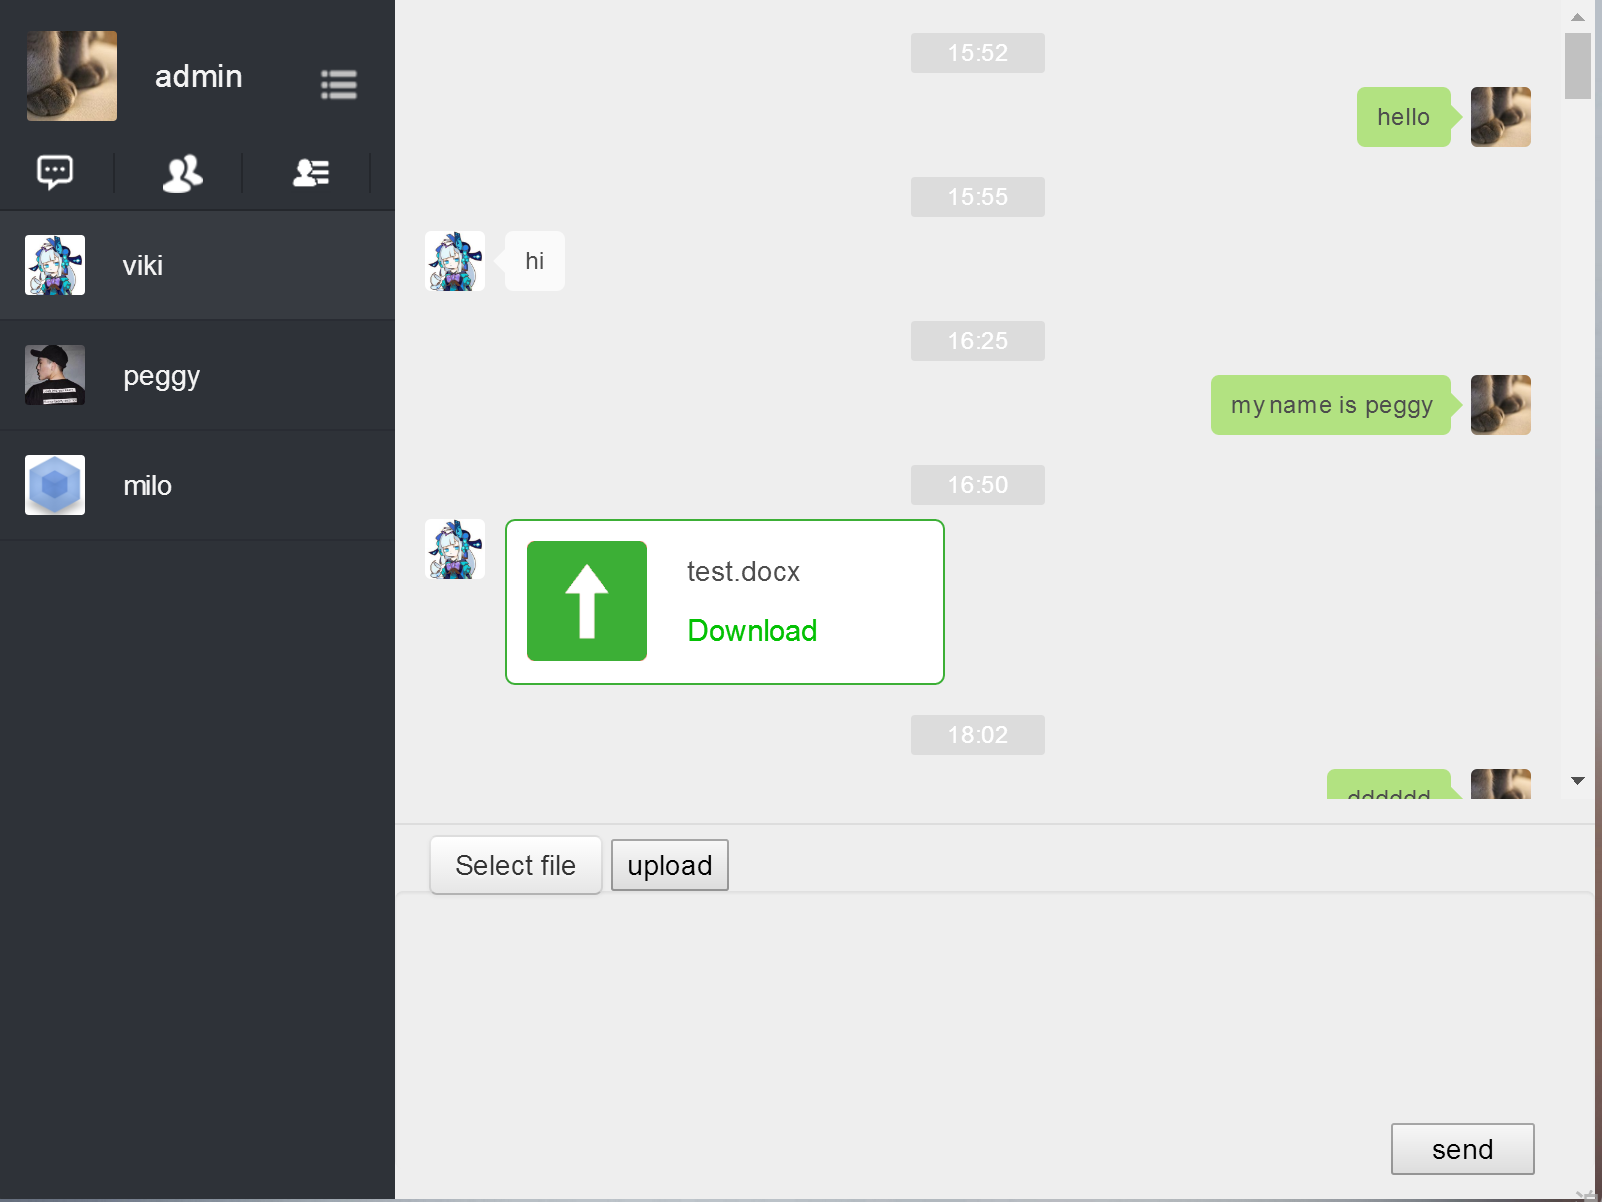
\includegraphics[width = 0.9 \textwidth ]{maininterface.png}
\caption{\label{fig:UML}Main Interface}
\end{figure}

\subsubsection*{Controller Tier}
The function of controller tier is connecting the model tier and the view tier in software. Therefore, it is used to communicate between the view tier and the model tier. Specifically, when a user action happened, it transfers data from related views to corresponding models. After that, when controller receive notifies from models, controller require views to update the information which should appear on the views. 

\subsubsection*{Model Tier}
The model manages fundamental behaviors and data of the application. On the one hand, it obtains the data of users action from the controller, and then, it responds to instructions that changing the state of information. Therefore, It can notify the user in event-driven systems when information changes. On the other hand, it could ask database, or data structures or storage systems for updating the data.

The infrastructure of web client is totally different with windows client. One of the most important aspects is that model tier can directly connection to database instead of getting data from the server. In view of this point, we have created a local database which is connected to model tier. All the relevant data will be gained from the main database and stored in the local database when user login. Furthermore, all those data will be deleted after logging off. 

\begin{lstlisting}[language=php]
//CREAT TABLE USER

public function createUser($tablename)
    {
        $sql="CREATE TABLE ".$tablename."(UserId INT NOT NULL,UserName VARCHAR (255) NOT NULL,PIN  VARCHAR(255) NOT NULL,profile  CHAR (255), Ip CHAR(255), PRIMARY KEY (UserId));";
        return $this->db->query($sql);
}
\end{lstlisting}
\begin{lstlisting}[language=php]
//DELETE USER TABLE
    public function deleteUser()
    {
        $query = $this->db->query('delete from user');
        return $query;
    }
\end{lstlisting}
\begin{lstlisting}[language=php]
//INSERT  BROADCAST user TALBE
    public function insertUUser($UserName,$info)
    {
        return $this->db->insert("".$UserName."", $info);
    }
\end{lstlisting}

\subsubsection{Function}
\subsubsection*{Registration}
In terms of registration, if users want to register a new account, the username, password and profile should be input. At first, web client will check whether the username has existed or not, because the username is used to identify the typical user. After checkout, those data will be inserted into the database.
\begin{lstlisting}[language=javascript]
 if(strs[0] == "register")
                {
                    conn.query('select * from user where UserName="'+strs[1]+'"',
                    function(err, rows, fields) {
                    if (err) throw err;
 if(rows.length>0){
                  obj="please change another username";
                  var json = JSON.stringify({type: 'register', data: obj});
                  clients[index].sendUTF(json);
                  }else
                       {
                        obj="succeed";
                        var json = JSON.stringify({type: 'register', data: obj});
                        clients[index].sendUTF(json);
                       }
\end{lstlisting}
\begin{figure}[!h]
\centering
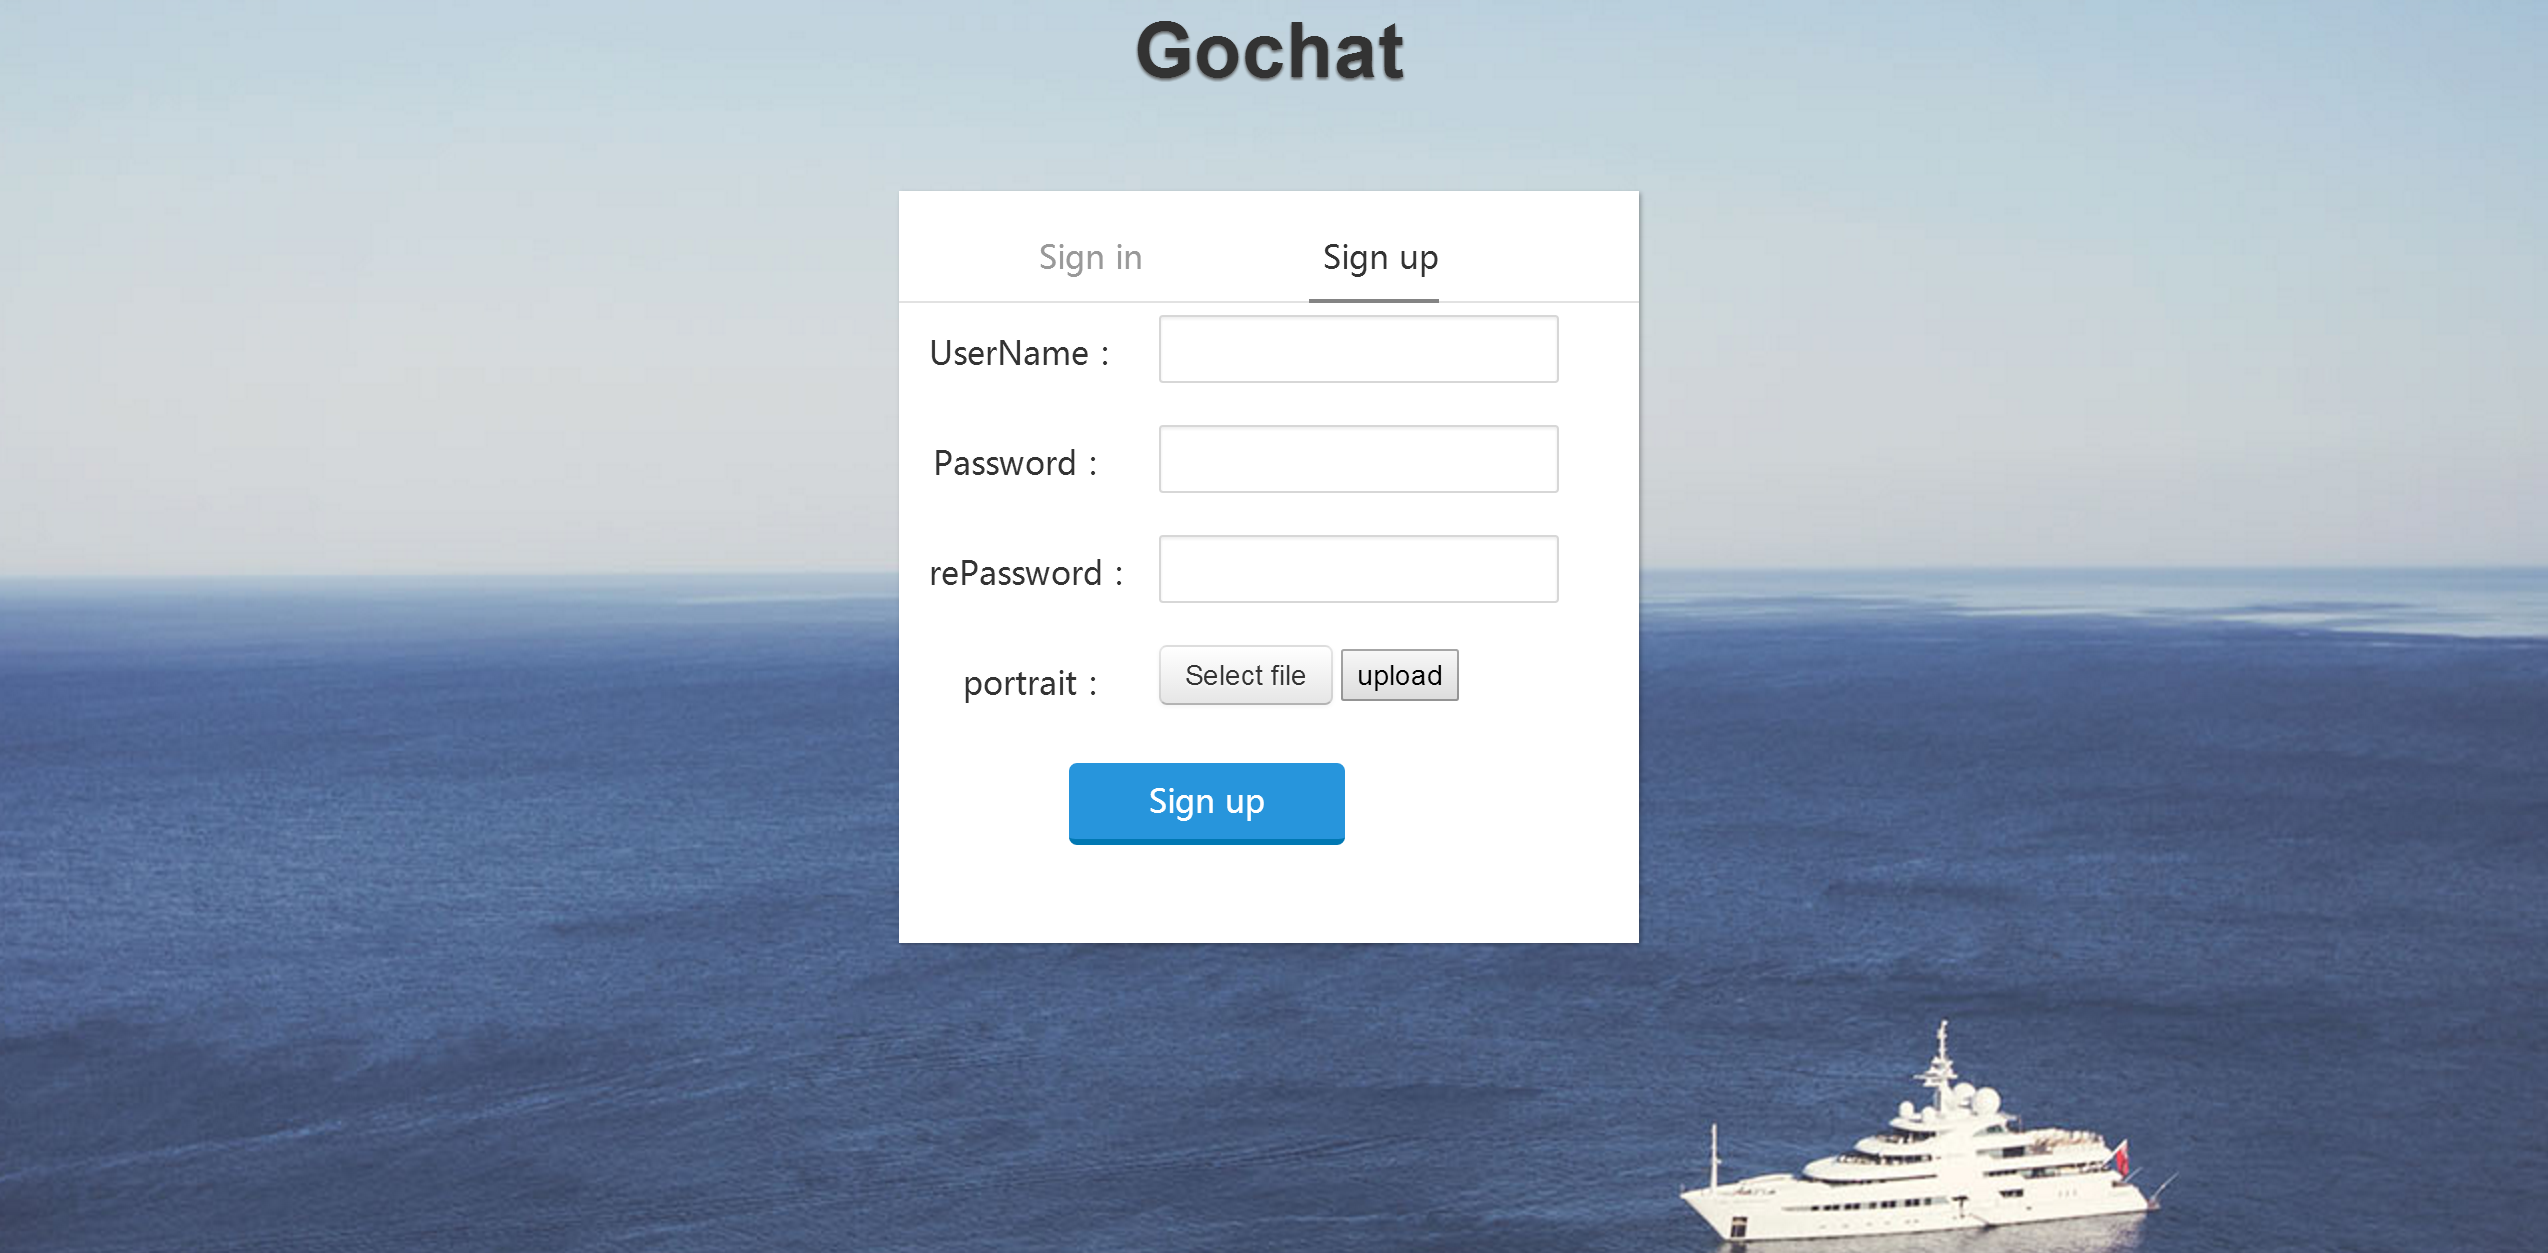
\includegraphics[width = 0.9 \textwidth ]{register.png}
\caption{\label{fig:UML}Registration}
\end{figure}

\subsubsection*{Chatting}
The most important aspect in Chatting function is how to send the message to server and how to define the type of the message. When User clicks the sending button, web client will send a request to server to build the connection. The message should be sent in the format of JSON, and the temple should be as following code.   
\begin{lstlisting}[language=javascript]
var str="message$"+ChatId+"$"+time+"$"+leftText+"$"+userId+"$0";
\end{lstlisting}
Before sending the JSON message to server, web client should parse it in order to judge whether it is a valid JSON, which is using JSON.parse()method. If the JSON message is valid, it will be inserted into the database and sent to target user. 
\begin{lstlisting}[language=javascript]
try {
        var json = JSON.parse(message.data);
        } catch (e) {
            console.log('This doesn\'t look like a valid JSON: ', message.data);
            return;
        }
        console.log(json);
        if (json.type === 'message') { 
            var message=json.data;
            var checkPwdURL = "/gochat/user/insertUMessage";
            }
\end{lstlisting}

\subsubsection*{Create Group Chatting}
For creating group chatting, we use the checkbox to list the option of friend list. Using checkbox is able to make sure user can choose several friends at same time. After clicking the confirmation button, all the userId of selected friends will be got by web client and joint it to a string named ‘apiContentStr’ using ‘for’ loop. Finally, the userId of the user should be added in front of the string and send this message to server. 
\begin{lstlisting}[language=javascript]
 createGroupChat.click(function() {
        var userId = document.getElementById('getUserId').value;
        var group = document.getElementsByName("contact");
        var objArray = group.length;
        var apiContentStr="";
        for(var i=0;i<objArray;i++){
            if(group[i].checked == true){
                apiContentStr += group[i].value+",";
            }
        }
        var member = apiContentStr.substring(0, apiContentStr.length - 1);
        member=userId+","+member;
        var str="chat$"+member+"$1";
        connection.send(str);
    });
\end{lstlisting}
\begin{figure}[!h]
\centering
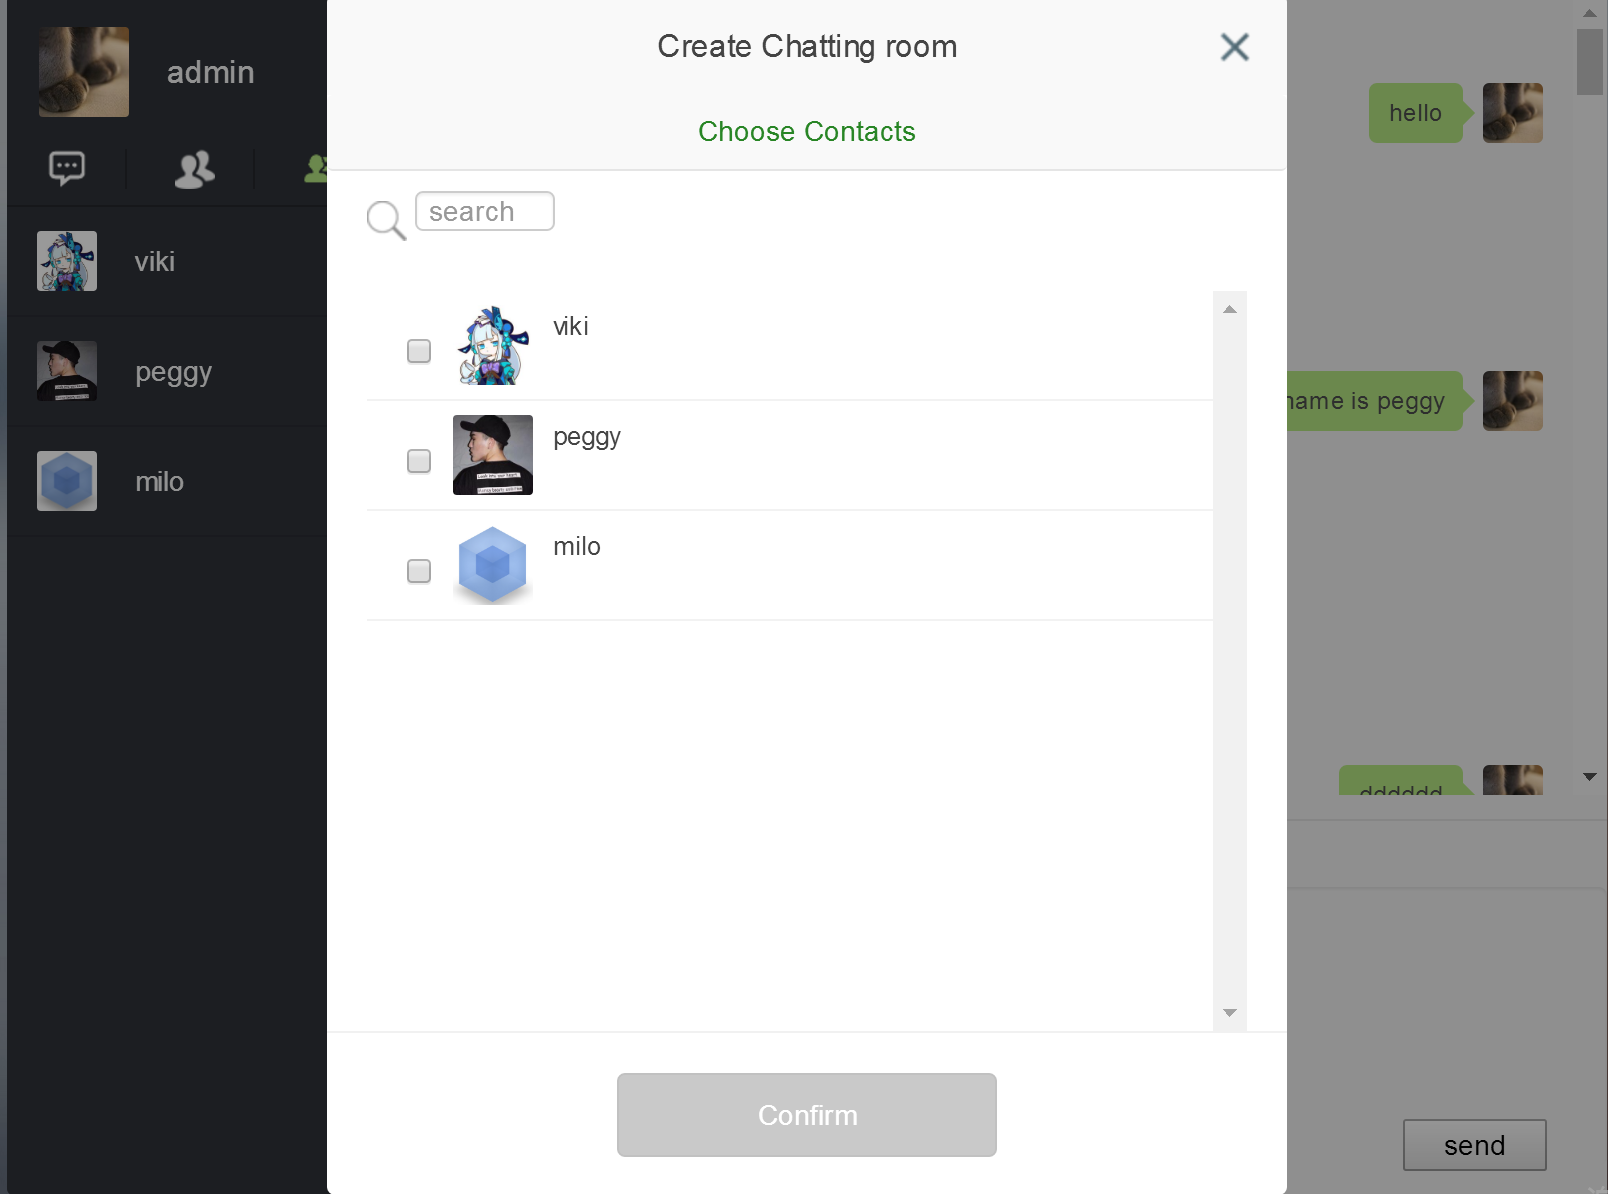
\includegraphics[width = 0.9 \textwidth ]{creategroupchat.png}
\caption{\label{fig:UML}Create Group Chat}
\end{figure}

\subsubsection*{Add Friend}
The process of adding friend is quite similar with Creating group chat. When user input the username and click the button, the web client will check whether the username exists or not. if it failed, web client will return an alert. On the contrary, the username and profile of target user will be displayed. For next step, web client will send the message to server in the following format after clicking the button of 'add'.
\begin{lstlisting}[language=javascript]
SFButton.click(function() {
        var userId = document.getElementById('getUserId').value;
        var FriendName = document.getElementById('searchusername').value;
        var str="search$"+userId+"$"+FriendName;
        connection.send(str);
    });
\end{lstlisting}

\begin{figure}[!h]
\centering
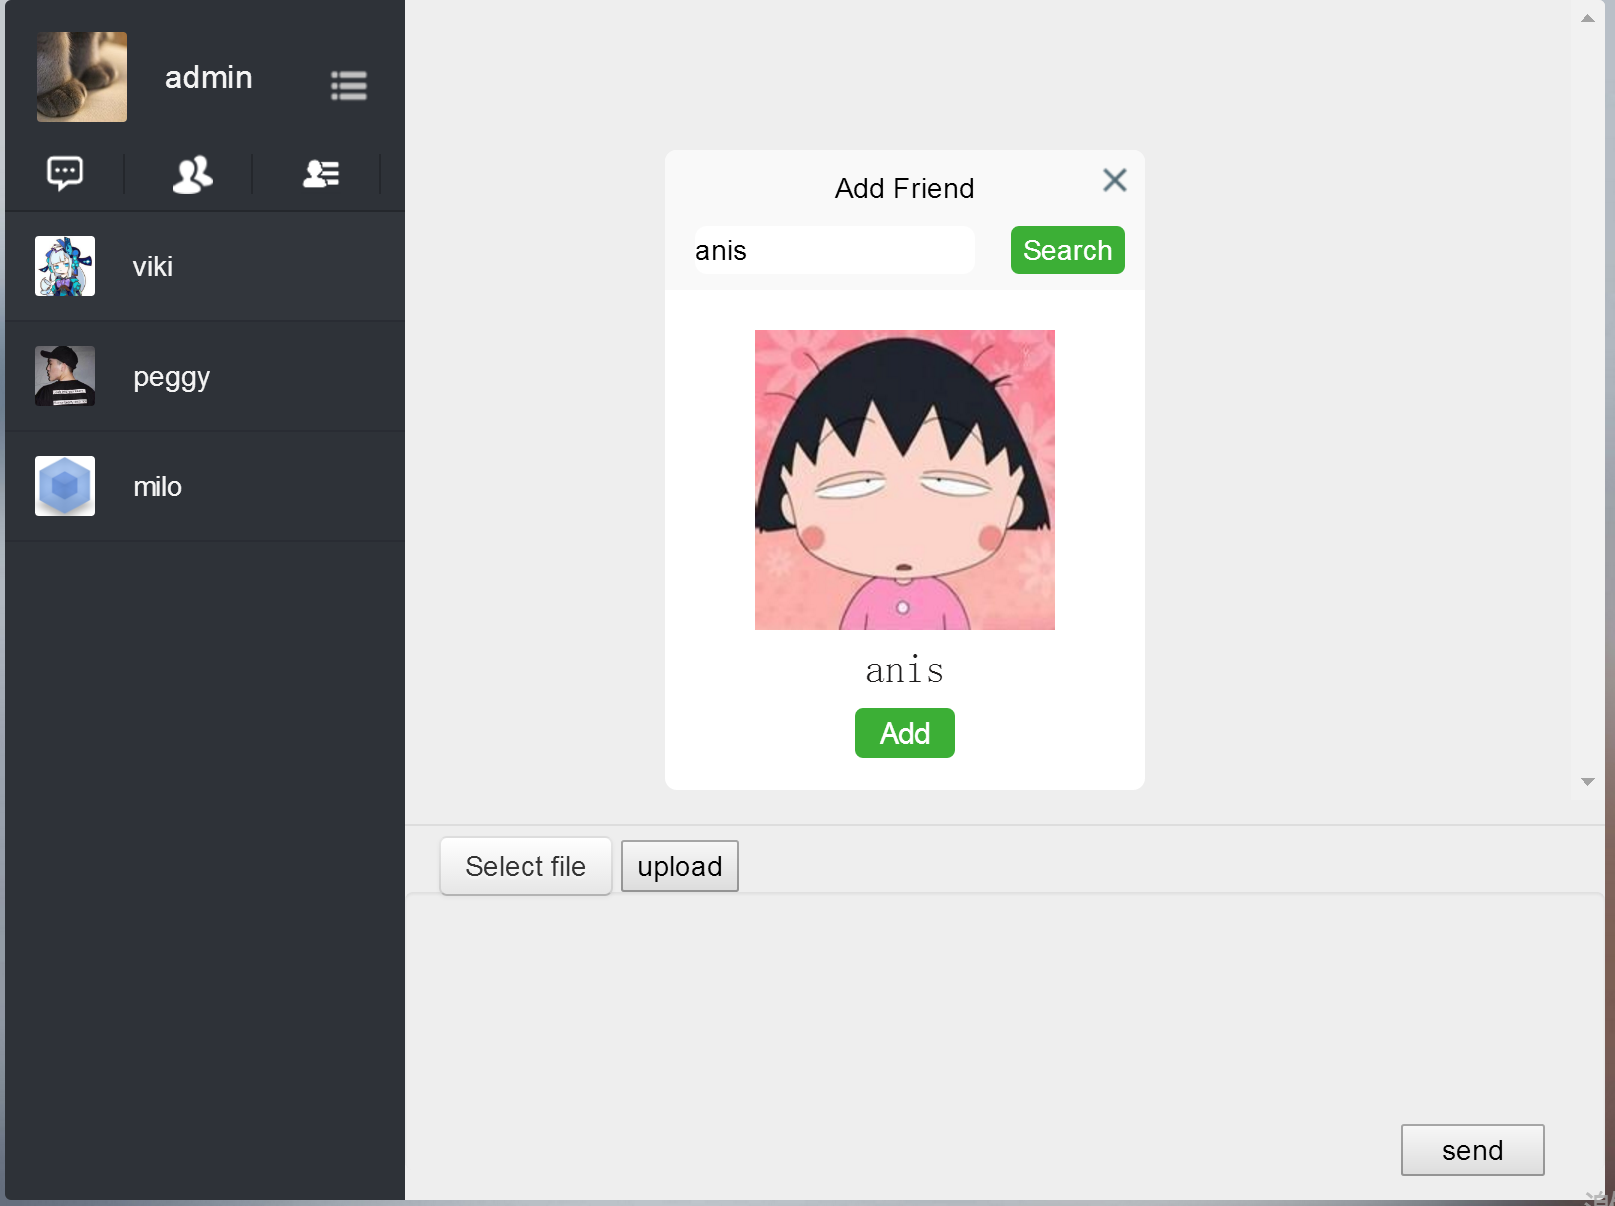
\includegraphics[width = 0.9 \textwidth ]{addfriendweb.png}
\caption{\label{fig:UML}Add Friends}
\end{figure}
\subsubsection*{Connection with Server}
If web client wants to connect the server, it will create a new socket at first. Then the client will try to connect to server through identifying the IP address of server and the port number. 
\begin{lstlisting}[language=javascript]
window.WebSocket = window.WebSocket || window.MozWebSocket;
connection = new WebSocket('ws://47.91.75.150:1337');
\end{lstlisting}
After connecting the server, the web client can monitor the message sent by server in real time by the function of ‘connection.onmessage’ if it keeps connecting to server. The function of ‘connection.onmessage’ can identify the type of the received message and execute the following command. 
\begin{lstlisting}[language=javascript]
connection.onmessage = function (message) {
 if (json.type === 'message') {
            var message=json.data;
            var checkPwdURL = "/gochat/user/insertUMessage";
                               }
                             }
\end{lstlisting}
\subsubsection*{Upload File or Image}
How to store the uploaded file in server in the most significant process to achieve the function of upload file and image. After user click the button to upload the file, controller will get the username of the sender, and set the path of this file as follow code:
\begin{lstlisting}[language=php]
 $filePath='./uploads/'.$UserName."/";
\end{lstlisting}
After server receives the path and file, the file should be stored in the ‘upload’ folder which will be created automatically if it does not exist in server. For the path, server will insert it into the database. The user who wants to download the file can get the path and find the target file in the folder of 'upload'.
\begin{lstlisting}[language=php]
 if (!file_exists($filePath))
        {
            mkdir ($filePath);
        }
\end{lstlisting}

\subsection{Test}

In windows application, functional test and common debug methods are taken to test functionalities and units of codes of our application. While new methods are added to the codes, try and catch methods (as following) and also are used to record the exception. Debug.writeline method is also used to debug our codes.
\begin{lstlisting}[language=C]
 try
            {
                set_loading();
                await socket.ConnectAsync(new Uri(wsUri), cts_timer.Token);
            }
            catch (Exception e)
            {
                ResetConnection();
                Debug.WriteLine("socket open error");
            }
\end{lstlisting}


For the functional testing part, six test tables are generated for testing six functions including login, sign up, sending messages, receiving messages, adding friends and creating new groups. As shown below, in both window and web clients, all functions work as our expectation.  

\begin{table}[h!]

\small
  \caption{Login Function Test Table}
\begin{tabular}{|c|l|c|c|c|c|c|c|c|c|c|c|}
 \hline

  \label{tab:table1}

   User Action & Expected Result & Result(web) & Result(window)\\ 
    \hline
       

    Don't type in username  & Msg: Type user name & Y & Y\\ \hline
 
      Don't type in passwd  & Msg: Type password & Y & Y\\ \hline
   
        Type wrong username or passwd & Msg: Wrong password & Y & Y\\ \hline
        Type right username and passwd & Pop up chat form & Y & Y \\ \hline
  \end{tabular}
\end{table}



\begin{table}[h!]
\centering
\small
  \caption{Sign Up Function Test Table}
\begin{tabular}{|c|l|c|c|c|c|c|c|c|c|c|c|}
 \hline
  \label{tab:table1}
    User Action & Expected Result & Result(web) & Result(window)\\ 
    \hline
   Don’t choose an image  & Msg: choose images & Y & Y\\ \hline
 
       Don’t type username & Msg: Type username & Y & Y\\ \hline
      Don't type passwd & Msg: Type passwd  & Y & Y\\ \hline
        Don't re-type passwd & Msg: Re-type passwd & Y & Y\\ \hline
        Re-type different passwd & Msg:type the same passwd & Y & Y \\ \hline
       Fill in all right info & Pop up login form & Y & Y \\ \hline
  \end{tabular}
\end{table}

\begin{table}[h!]
\centering
\small
  \caption{Send Messages Function Test Table}
\begin{tabular}{|c|l|c|c|c|c|c|c|c|c|c|c|}
 \hline
  \label{tab:table1}
      User Action & Expected Result & Result(web) & Result(window)\\ 
    \hline
   Don’t type any msg and click send  & No msg show out & Y & Y\\ \hline
 
    type msg and send & Msg show out & Y & Y\\ \hline
    
  \end{tabular}
\end{table}

\begin{table}[h!]
\centering
\small
  \caption{Receive Messages Function Test Table}
\begin{tabular}{|c|l|c|c|c|c|c|c|c|c|c|c|}
 \hline
  \label{tab:table1}
      User Action & Expected Result & Result(web) & Result(window)\\ 
    \hline
  Friends send messages  & Msg show out & Y & Y\\ \hline
  \end{tabular}
\end{table}

\begin{table}[h!]
\centering
\small
  \caption{Add Friends Function Test Table}
\begin{tabular}{|c|l|c|c|c|c|c|c|c|c|c|c|}
 \hline
  \label{tab:table1}
      User Action & Expected Result & Result(web) & Result(window)\\ 
    \hline
   Don’t type in search info and click search  & Msg: info should not be empty & Y & Y\\ \hline
    Type in search info and click search & User name and image show out & Y & Y\\ \hline
  \end{tabular}
\end{table}


\begin{table}[h!]
\centering
\small
  \caption{Create New Groups Function Test Table}
\begin{tabular}{|c|l|c|c|c|c|c|c|c|c|c|c|}
 \hline
  \label{tab:table1}
      User Action & Expected Result & Result(web) & Result(window)\\ 
    \hline
   Don’t click any friends or groups  & Msg: select friends or groups & Y & Y\\ \hline
 
   Click friends or group & New group shows in group list & Y & Y\\ \hline
    
  \end{tabular}
\end{table}




\section{Team Work}
We divided the whole development life cycle of our group project to three phases. 

The first phase is designing that was done in the first two weeks of this project. The six of us met together more than 6 hours per week and everyone stated their opinions and views in our group discussion. In the end of the first phases, we had done the initial design and requirement for our project.

The second phase is programing and the period of it is from February 13 to March 29. We divided our team member into two small teams, web application team and window application team. The first team includes Chen Huiping, Chen Jin and Li Yiqi, who build the web client. While the rest of the member are (Park Woomin, Anisaul Muawwanah and Chen Wenwen) responsible for the window client. Our two team worked together, we worked at least 10 hours peer week at group study room in the library.

The last phase is testing and documentation. While the testing basically happened the whole time we did the programming, the documentation was started at the last two weeks. Our member were separated into two small teams. One is main programmer team, they (Park Woomin, Chen Huiping, and Anisaul Muawwanah) build the server, link our clients with the server and solve the bugs. While Chen Wenwen, Chen Jin and Li Yiqi are in another group. They optimize the interface, in charge of the security part, do black and white test of our application. Our two teams also worked together in this period and we worked more than 12 hours peer week at group meeting room in the library.


\section{Evaluation}


\subsection{Advantage}
In our project, websocket is a protocol chosen by us for communication.Even though our security has not been completed, using TLS over websocket will give us a much easier and securer way to achieve security goal. And also, in our future work, if we want to realize video chatting, websocket is helpful and useful due to its attribute. 

Since we have finished our basic functions of the chatting system, users could easily create a account in our system and login in web pages and also windows desktop application. After that, they could send pictures, images and documents to their friends whenever and wherever they want. Additionally, they could add new friends once they find out another friends also using our system. A group chat is also able to be added to begin a group talk and share files.  

\subsection{Disadvantage}
 
\subsubsection{Server}

With more researches about Apache server going on, we found out that Apache server can not communicate with window client. And then, we tried to design a window desktop server instead according to demonstrations and references found online. But after having the server running, we found out the web client can not receive messages from the server continuously. While spending time to solve the problem in the window desktop server, we were also doing researches about web server.   Since the window desktop server problem can not be fixed and a web server used Javascript as programming language achieved our goal, communicating with both window client and web client using WebSocket protocol, the web server was built and chose at the end.  

 
\subsubsection{Windows Client}
The client part is slightly changed. When client 1 sends files or images, the client will firstly send file path in a given format to the server. By the meantime, the file is uploaded to the specific folder in the server. After that, the server will send the file path to client 2.

At the beginning, list form and message form are combined together. But every time when users click one of their friends, the user control item is called so frequently to display the chatting history that all messages flash in the first several seconds. Thus, we decided to separate list form and message form. Only after all chatting history has been loaded and shown out, the message form will be pop up. 


When we ran the application with checking it in task manager, it is found out that too much resources have been used and around 50\% of CPU have been occupied by the chat application. After debugging the whole application, it showed that the reason comes from that a thread is running on background and checking whether WebSocket connection flag is true ( it will be set to true when users click close button in chatting form) and if it is true, it will cancel the existing connection. This requires numerous resources. 
\begin{lstlisting}[language=C]
while (true)
            {
                if (ws_socket_flag)
                {
                    cts.Cancel();
                    return;
                }
            }
\end{lstlisting}
To improve our application, another function is defined and used to reset connection when users click close button in chatting form instead of using while statement. With calling this function, stored data in memory is cleared. Background worker is disposed and cancel token resources and WebSocket client are reset to ensure no unnecessary threads running in the background and Websocket connection is reset. 
\begin{lstlisting}[language=C]
public void ResetConnection()
        {
                initTable();
                StartWSClient.Dispose();
                cts.Cancel();
                cts = null;
                socket = null;
        }

\end{lstlisting}



\subsubsection{Web Client}
After connecting our web client with the database, we have found an obvious question. The client could obtain and change the data directly from the main database, when the connection between web clients and the main database was built, as our web client was based on Model, View and Controller (MVC) structure. After our discussed, we think that our web clients should build the connection with servers rather than main database. In this way, our web clients could send requires to the server for acquiring and changing information from the database. However, of our web clients is not available for the type of connection, because the model tier only connectives with database in the MVC structure. On the other hand, we have already done the majority of codes, so we do not have enough time to change the structure of our web clients. For this reason, we have to create a local database which is use to download the data of the user who log in at present. It demonstrates that when a user login, the web client of user send require automatically, download all user’s data from main database and save these data in the new local database. Therefore, users can use data from the local database, but the local database will be deleted if the user logs out. 
After we finished the local database part, we found another problem. If one user login, the web clients will download the related data about that user, including their friends’ username and Id. However, one of the users’ friends login at the same web client again. Too many information will be download and save into local database again. In this way, if too many users log in, too many user information will be copied multiple times, so it affects other function in the web client. Our solution is that creating four data table for each user. The structure of the tables is same as tables which are from main database. But the name of the table is changed as following: 'user+username','chat+username' etc. the four table will be deleted if the user logs out. Although this method solves this problem basically, it will still cause a huge number of tables exist in the database if lots of users online at same time.

\begin{figure}[!h]
\centering
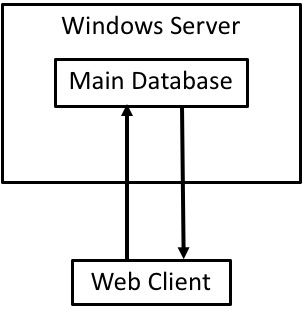
\includegraphics[width = 0.5 \textwidth ]{previous_vision.jpeg}
\caption{\label{fig:UML}Previous Vision}
\end{figure}
\begin{figure}[!h]
\centering
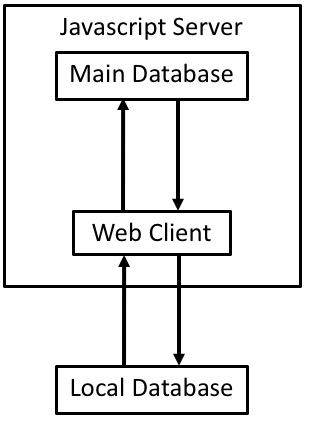
\includegraphics[width = 0.5 \textwidth ]{current_vision.jpeg}
\caption{\label{fig:UML}Current Vision}
\end{figure}
\subsection{Advantage}
Due to the limitation of time, the function that users could delete their chatting history and customize their chatting history expire time to prevent data theft has not been done. 

In communication security part, Elliptic curve Diffie-Helmen key exchange and AES key encryption is used because of time limitation. 


\subsection{Time management}

During the week that we submit our initial report and presentation, we began to install visual studio 2017 and PHP storm and also configured our laptops like XAMPP for using these tools. After that, we started to develop basic chatting function for our system. Due to the change of our server as mentioned in the evaluation part, our clients codes have to be altered as well, which caused us to spend double time on level 1 basic chatting program and level 2 security part. And also at the end, we didn't have enough time to apply other additional functions.    

\definecolor{No}{RGB}{255,255,185}
\definecolor{UML}{RGB}{205,205,180}
\definecolor{Data}{RGB}{205,205,180}
\definecolor{intermediate}{RGB}{205,205,180}
\definecolor{environ}{RGB}{205,205,180}
\definecolor{level1}{RGB}{205,205,180}
\definecolor{level2}{RGB}{205,205,180}
\definecolor{level3}{RGB}{205,205,180}
\definecolor{debug}{RGB}{205,205,180}
\definecolor{documentation}{RGB}{205,205,180}
\definecolor{final}{RGB}{205,205,180}
\begin{table}[h]
\centering
\caption{Task time table (Initial)}
\label{my-label}
\begin{tabular}{|c|l||c|c|c|c|c|c|c|c|c|c|}
\hline
\rowcolor{No}
No. & Task name & 01 & 02 & 03 & 04 & 05 & 06 & 07 & 08 & 09 & 10 \\ \hline \hline
1 & UML design & \cellcolor{UML} & \cellcolor{UML} &  &  &  &  &  &  &  &  \\ \hline
2 & Database design & \cellcolor{Data} & \cellcolor{Data} &  &  &  &  &  &  &  &  \\ \hline
3 & Intermediate report \& presentation &  & \cellcolor{intermediate} & \cellcolor{intermediate} &  &  &  &  &  &  &  \\ \hline
4 & Developing environment setting &  &  & \cellcolor{environ} & \cellcolor{environ} &  &  &  &  &  &  \\ \hline
5 & Level 1: basic chatting program &  &  & \cellcolor{level1} & \cellcolor{level1} & \cellcolor{level1} &  &  &  &  &  \\ \hline
6 & Level 2: security &  &  &  &  & \cellcolor{level2} & \cellcolor{level2} & \cellcolor{level2} &  &  &  \\ \hline
7 & Level 3: Other additional function &  &  &  &  &  &  & \cellcolor{level3} & \cellcolor{level3} & \cellcolor{level3} &  \\ \hline
8 & Debug &  &  &  &  & \cellcolor{debug} & \cellcolor{debug} & \cellcolor{debug} & \cellcolor{debug} & \cellcolor{debug} & \cellcolor{debug} \\ \hline
9 & Documentation &  &  &  &  & \cellcolor{documentation} &  & \cellcolor{documentation} &  & \cellcolor{documentation} &  \\ \hline
10 & Final report \& presentation &  &  &  &  &  &  &  &  & \cellcolor{final} & \cellcolor{final} \\ \hline
\end{tabular}
\end{table}

\definecolor{No}{RGB}{255,255,185}
\definecolor{UML}{RGB}{205,205,180}
\definecolor{Data}{RGB}{205,205,180}
\definecolor{intermediate}{RGB}{205,205,180}
\definecolor{environ}{RGB}{205,205,180}
\definecolor{level1}{RGB}{205,205,180}
\definecolor{level2}{RGB}{205,205,180}
\definecolor{level3}{RGB}{205,205,180}
\definecolor{debug}{RGB}{205,205,180}
\definecolor{documentation}{RGB}{205,205,180}
\definecolor{final}{RGB}{205,205,180}
\begin{table}[h]
\centering
\caption{Task time table (Last)}
\label{my-label}
\begin{tabular}{|c|l||c|c|c|c|c|c|c|c|c|c|}
\hline
\rowcolor{No}
No. & Task name & 01 & 02 & 03 & 04 & 05 & 06 & 07 & 08 & 09 & 10 \\ \hline \hline
1 & UML design & \cellcolor{UML} & \cellcolor{UML} &  &  &  &  &  &  &  &  \\ \hline
2 & Database design & \cellcolor{Data} & \cellcolor{Data} &  &  &  &  &  &  &  &  \\ \hline
3 & Intermediate report \& presentation &  & \cellcolor{intermediate} & \cellcolor{intermediate} &  &  &  &  &  &  &  \\ \hline
4 & Developing environment setting &  &  & \cellcolor{environ} &  &  &  &  &  &  &  \\ \hline
5 & Level 1: basic chatting program &  &  &  & \cellcolor{level1} & \cellcolor{level1} & \cellcolor{level1}  & \cellcolor{level1} & \cellcolor{level1}  &  &  \\ \hline
6 & Level 2: security &  &  &  &  & &  & \cellcolor{level2}  & \cellcolor{level2}  & \cellcolor{level2} &  \cellcolor{level2} \\ \hline
7 & Level 3: Other additional function &  &  &  &  &  &  &  &  &  &  \\ \hline
8 & Debug &  &  &  &  & \cellcolor{debug} & \cellcolor{debug} & \cellcolor{debug} & \cellcolor{debug} & \cellcolor{debug} & \cellcolor{debug} \\ \hline
9 & Documentation &  &  &  &  & \cellcolor{documentation} &  & \cellcolor{documentation} &  & \cellcolor{documentation} &  \\ \hline
10 & Final report \& presentation &  &  &  &  &  &  &  &  & \cellcolor{final} & \cellcolor{final} \\ \hline
\end{tabular}
\end{table}




\subsection{Future Work}
The application that we build is not a complete version. There are a number of issues that need to be addressed to make this application better, such as the security and additional functions to make the application more enjoyable.

In the start of our project, we planned to build a secure chat system. Unfortunately, we were only able to finish the hashing part to secure stored passwords. This indeed helps protect the application from attackers who want to get the password, but it did not help to secure the communication between client-server. Attacker can easily read our messages because they are all send as plain text. This issue need to be addressed as soon as possible for confidentiality purpose. It is our intention to add encryption function to secure the communication between client-server. We consider to use AES as encryption algorithm and CBC as mode of operation. In fact, we already tried to implement them, but there were some error that we could not solved for now.

Regarding the security, we also believe that we should develop our own library to handle the security problems, such as hashing and encrypting. In this project, we use 'node-forge' library provided by 'digitalbazaar'. In one hand, this decision seems to be a wise choice because we use a trusted library that has been tested by people. On the other hand, using a library for security means that we must trust this library to secure our system. That is like putting a lot of trust into another person. And this could turn out to be really bad if we do not understand the source codes used in the library. Meanwhile, developing our own library means building the codes ourself. So, we put the faith of security into our hand. It is true that building this library might need a lot of time because of our limited knowledge and experience. We might have to involve a lot of people to review and test out codes. But we believe that this could be a challenging and worthy work.

Another problem that need to be solved is the additional functions that supposed to make the application more enjoyable for user. Fun features, such as using emojis, gif, drawing picture, and image compose, should be added to the application.


\section{Peer assessment}
We believe that we as the member of the group have the same responsibilities for the success of our project. We firmly believe that each of our members will work as hard as they can to ensure this project is a success. That is why we decided to give each of us a 15 mark for our effort. On the other hand, we will divide the rest of 10 marks based on our member’s creativity, ability to handle stress and pressure, and capacity to keep our group together. 

After discussing with our group members, our group would like to give Chen Huiping and Park Woomin extra 3 marks separately, so it means they (Chen Huiping and Park Woomin) both get 18 marks. The reason is that they play the part of leader in our group project, because they have lots of experience in programming and show their willing to teach other teammates. They are not only can finish their assignment early, but also encourage and give hand to other teammates. Therefore, our group be able to finish our group project successfully. While, other four teammates (Li Yiqi, Chen Jing, Chen Wenwen and Anisaul Muawwanah) get extra 1 mark as encouragement separately, because they aggressive and want to learn and also try their best when they do their assignments. Therefore, these four teammates are marked 16 marks.











\end{document}